%%%%%%%%%%%%  Generated using docx2latex.com  %%%%%%%%%%%%%%

%%%%%%%%%%%%  v2.0.0-beta  %%%%%%%%%%%%%%

\documentclass[12pt]{article}
\usepackage{amsmath}
\usepackage{latexsym}
\usepackage{amsfonts}
\usepackage[normalem]{ulem}
\usepackage{array}
\usepackage{amssymb}
\usepackage{graphicx}
\usepackage[backend=biber,
style=numeric,
sorting=none,
isbn=false,
doi=false,
url=false,
]{biblatex}\addbibresource{bibliography.bib}

\usepackage{subfig}
\usepackage{wrapfig}
\usepackage{wasysym}
\usepackage{enumitem}
\usepackage{adjustbox}
\usepackage{ragged2e}
\usepackage[svgnames,table]{xcolor}
\usepackage{tikz}
\usepackage{longtable}
\usepackage{changepage}
\usepackage{setspace}
\usepackage{hhline}
\usepackage{multicol}
\usepackage{tabto}
\usepackage{float}
\usepackage{multirow}
\usepackage{makecell}
\usepackage{fancyhdr}
\usepackage[toc,page]{appendix}
\usepackage[hidelinks]{hyperref}
\usetikzlibrary{shapes.symbols,shapes.geometric,shadows,arrows.meta}
\tikzset{>={Latex[width=1.5mm,length=2mm]}}
\usepackage{flowchart}\usepackage[paperheight=11.69in,paperwidth=8.27in,left=1.18in,right=1.18in,top=0.98in,bottom=0.98in,headheight=1in]{geometry}
\usepackage[utf8]{inputenc}
\usepackage[T1]{fontenc}
\TabPositions{0.49in,0.98in,1.47in,1.96in,2.45in,2.94in,3.43in,3.92in,4.41in,4.9in,5.39in,5.88in,}

\urlstyle{same}


 %%%%%%%%%%%%  Set Depths for Sections  %%%%%%%%%%%%%%

% 1) Section
% 1.1) SubSection
% 1.1.1) SubSubSection
% 1.1.1.1) Paragraph
% 1.1.1.1.1) Subparagraph


\setcounter{tocdepth}{5}
\setcounter{secnumdepth}{5}


 %%%%%%%%%%%%  Set Depths for Nested Lists created by \begin{enumerate}  %%%%%%%%%%%%%%


\setlistdepth{9}
\renewlist{enumerate}{enumerate}{9}
		\setlist[enumerate,1]{label=\arabic*)}
		\setlist[enumerate,2]{label=\alph*)}
		\setlist[enumerate,3]{label=(\roman*)}
		\setlist[enumerate,4]{label=(\arabic*)}
		\setlist[enumerate,5]{label=(\Alph*)}
		\setlist[enumerate,6]{label=(\Roman*)}
		\setlist[enumerate,7]{label=\arabic*}
		\setlist[enumerate,8]{label=\alph*}
		\setlist[enumerate,9]{label=\roman*}

\renewlist{itemize}{itemize}{9}
		\setlist[itemize]{label=$\cdot$}
		\setlist[itemize,1]{label=\textbullet}
		\setlist[itemize,2]{label=$\circ$}
		\setlist[itemize,3]{label=$\ast$}
		\setlist[itemize,4]{label=$\dagger$}
		\setlist[itemize,5]{label=$\triangleright$}
		\setlist[itemize,6]{label=$\bigstar$}
		\setlist[itemize,7]{label=$\blacklozenge$}
		\setlist[itemize,8]{label=$\prime$}

\setlength{\topsep}{0pt}\setlength{\parskip}{8.04pt}
\setlength{\parindent}{0pt}

 %%%%%%%%%%%%  This sets linespacing (verticle gap between Lines) Default=1 %%%%%%%%%%%%%%


\renewcommand{\arraystretch}{1.3}


%%%%%%%%%%%%%%%%%%%% Document code starts here %%%%%%%%%%%%%%%%%%%%



\begin{document}


%%%%%%%%%%%%%%%%%%%% Figure/Image No: 1 starts here %%%%%%%%%%%%%%%%%%%%

\begin{figure}[H]
	\begin{Center}
		\includegraphics[width=1.92in,height=2.24in]{./media/image1.pdf}
	\end{Center}
\end{figure}


%%%%%%%%%%%%%%%%%%%% Figure/Image No: 1 Ends here %%%%%%%%%%%%%%%%%%%%

\par

\begin{Center}
{\fontsize{18pt}{21.6pt}\selectfont \textbf{UNIVERSIDADE FEDERAL DA FRONTEIRA SUL}\par}
\end{Center}\par


\vspace{\baselineskip}

\vspace{\baselineskip}

\vspace{\baselineskip}

\vspace{\baselineskip}

\vspace{\baselineskip}

\vspace{\baselineskip}
\begin{Center}
{\fontsize{24pt}{28.8pt}\selectfont \textbf{LOGARITMOS E FUNÇÕES LOGARITMICAS}\par}
\end{Center}\par


\vspace{\baselineskip}
\begin{Center}
{\fontsize{16pt}{19.2pt}\selectfont Professores:\par}
\end{Center}\par

\begin{Center}
{\fontsize{20pt}{24.0pt}\selectfont \textbf{Pedro Augusto Pereira Borges}\par}
\end{Center}\par

\begin{Center}
{\fontsize{20pt}{24.0pt}\selectfont \textbf{Marisol Vieira Melo}\par}
\end{Center}\par


\vspace{\baselineskip}
\begin{Center}
{\fontsize{14pt}{16.8pt}\selectfont Colaborador:\par}
\end{Center}\par

\begin{Center}
{\fontsize{20pt}{24.0pt}\selectfont \textbf{Fernando Augusto Brancher}\par}
\end{Center}\par


\vspace{\baselineskip}

\vspace{\baselineskip}
\begin{Center}
\textbf{NOVEMBRO/2014}
\end{Center}\par


\vspace{\baselineskip}
\setlength{\parskip}{0.0pt}
\begin{enumerate}[label*={\fontsize{14pt}{14pt}\selectfont \textbf{\arabic*.}}]
	\item {\fontsize{14pt}{16.8pt}\selectfont \textbf{Porque foram criados e qual é a utilidade dos Logaritmos?}\par}\par


\vspace{\baselineskip}
\begin{justify}
\tab Um dos grandes desafios da matemática no fim do século XVI e início do XVII era o desenvolvimento de meios para facilitar os cálculos aritméticos, evitando erros grosseiros e objetivando o auxílio a outras ciências. Nesse período em especial, as ciências que impulsionaram esses desenvolvimentos foram, a astronomia, que estava em alta na época e a navegação, influenciada pelo comércio mundial. Foram criados diversos métodos para facilitar os cálculos na época, porém a maioria deles fracassou por serem praticamente inviáveis ou de pouca precisão. Os logaritmos, na sua origem, foram criados como um meio de simplificar complexas operações de multiplicação e divisão, transformando-as em simples adições e subtrações.
\end{justify}\par

\begin{justify}
\tab John Napier (1550-1617) e Jobst Bürgi (1552-1632) são considerados pais da ideia de logaritmos conhecida hoje. Os trabalhos de Napier e Bürgi foram desenvolvidos independentes e quase que simultaneamente e tiveram focos diferentes no decorrer de seus trabalhos. Enquanto Napier desenvolveu seu trabalho a partir de noções geométricas, Bürgi trabalhou baseando-se em noções algébricas. 
\end{justify}\par

\begin{justify}
\tab É importante salientar também a importância de Michael Stifel (1487-1567), considerado um dos principais precursores dos logaritmos. Stifel publicou em 1544 o livro \textit{Arithmetica integra}, publicação de extrema importância para a álgebra da Alemanha no século XVI. É nessa obra que aparece uma origem para a ideia de logaritmo. Stifel descobre as vantagens de se fazer a associação entre uma progressão geométrica e uma progressão aritmética, um século antes da invenção dos logaritmos. Ele observou que o produto (quociente) de dois termos quaisquer da progressão geométrica está associado à soma (diferença) dos correspondentes na progressão aritmética.
\end{justify}\par

\begin{justify}
\tab Napier não era matemático profissional. Além de cuidar da administração de suas propriedades, se dedicou a escrever sobre vários assuntos. O termo logaritmo foi criado por ele e vem do latim, \textit{logos = }razão e \textit{arithmos =} número.\textit{ }Esse método, era para Napier, uma tentativa de expressar o cálculo a partir da razão ou da proporção numérica. Foi no ano de 1614, três anos antes de sua morte e seis anos antes da publicação de Bürgi, que John Napier publicou sua descoberta na obra intitulada de \textit{Mirifici logarithmorum canonis descriptio} (ou seja, \textit{Uma descrição da maravilhosa regra dos logaritmos}). Nesse livro, Napier explica através de sua concepção, os logaritmos, e junto disso fornece uma tábua dos logaritmos dos senos de 0º a 90º, de minuto em minuto. O motivo de Napier ter aplicado sua ideia à trigonometria foi devido ao fato que a intenção da criação dessa tabua de logaritmos era facilitar os extensos e complicados cálculos realizados pelos astrônomos e navegadores. Baseado nas publicações de Stifel, Napier deparou-se com a evidência de que as somas ou diferenças dos índices das potências eram na verdade produtos ou quocientes das potências dadas.
\end{justify}\par

\begin{justify}
\tab Observando a tabela a seguir é possível compreender a conclusão a qual Napier chegou: 
\end{justify}\par


\vspace{\baselineskip}


%%%%%%%%%%%%%%%%%%%% Table No: 1 starts here %%%%%%%%%%%%%%%%%%%%


\begin{table}[H]
 			\centering
\begin{tabular}{p{0.07in}p{0.07in}p{0.07in}p{0.14in}p{0.14in}p{0.14in}p{0.21in}p{0.21in}p{0.21in}p{0.29in}p{0.29in}p{0.29in}p{0.29in}p{0.37in}p{0.37in}}
\hline
%row no:1
\multicolumn{1}{|p{0.07in}}{\cellcolor[HTML]{FFFFFF}\Centering {\fontsize{14pt}{16.8pt}\selectfont 1}} & 
\multicolumn{1}{|p{0.07in}}{\cellcolor[HTML]{FFFFFF}\Centering {\fontsize{14pt}{16.8pt}\selectfont 2}} & 
\multicolumn{1}{|p{0.07in}}{\cellcolor[HTML]{FFFFFF}\Centering {\fontsize{14pt}{16.8pt}\selectfont 3}} & 
\multicolumn{1}{|p{0.14in}}{\cellcolor[HTML]{FFFFFF}\Centering {\fontsize{14pt}{16.8pt}\selectfont 4}} & 
\multicolumn{1}{|p{0.14in}}{\cellcolor[HTML]{FFFFFF}\Centering {\fontsize{14pt}{16.8pt}\selectfont \textbf{\uline{5}}}} & 
\multicolumn{1}{|p{0.14in}}{\cellcolor[HTML]{FFFFFF}\Centering {\fontsize{14pt}{16.8pt}\selectfont 6}} & 
\multicolumn{1}{|p{0.21in}}{\cellcolor[HTML]{FFFFFF}\Centering {\fontsize{14pt}{16.8pt}\selectfont 7}} & 
\multicolumn{1}{|p{0.21in}}{\cellcolor[HTML]{FFFFFF}\Centering {\fontsize{14pt}{16.8pt}\selectfont 8}} & 
\multicolumn{1}{|p{0.21in}}{\cellcolor[HTML]{FFFFFF}\Centering {\fontsize{14pt}{16.8pt}\selectfont \textbf{\uline{9}}}} & 
\multicolumn{1}{|p{0.29in}}{\cellcolor[HTML]{FFFFFF}\Centering {\fontsize{14pt}{16.8pt}\selectfont 10}} & 
\multicolumn{1}{|p{0.29in}}{\cellcolor[HTML]{FFFFFF}\Centering {\fontsize{14pt}{16.8pt}\selectfont 11}} & 
\multicolumn{1}{|p{0.29in}}{\cellcolor[HTML]{FFFFFF}\Centering {\fontsize{14pt}{16.8pt}\selectfont 12}} & 
\multicolumn{1}{|p{0.29in}}{\cellcolor[HTML]{FFFFFF}\Centering {\fontsize{14pt}{16.8pt}\selectfont 13}} & 
\multicolumn{1}{|p{0.37in}}{\cellcolor[HTML]{FFFFFF}\Centering {\fontsize{14pt}{16.8pt}\selectfont \textbf{\uline{14}}}} & 
\multicolumn{1}{|p{0.37in}|}{\cellcolor[HTML]{FFFFFF}\Centering {\fontsize{14pt}{16.8pt}\selectfont 15}} \\
\hhline{---------------}
%row no:2
\multicolumn{1}{|p{0.07in}}{\cellcolor[HTML]{FFFFFF}\Centering 2} & 
\multicolumn{1}{|p{0.07in}}{\cellcolor[HTML]{FFFFFF}\Centering 4} & 
\multicolumn{1}{|p{0.07in}}{\cellcolor[HTML]{FFFFFF}\Centering 8} & 
\multicolumn{1}{|p{0.14in}}{\cellcolor[HTML]{FFFFFF}\Centering 16} & 
\multicolumn{1}{|p{0.14in}}{\cellcolor[HTML]{FFFFFF}\Centering \textbf{\textit{\uline{32}}}} & 
\multicolumn{1}{|p{0.14in}}{\cellcolor[HTML]{FFFFFF}\Centering 64} & 
\multicolumn{1}{|p{0.21in}}{\cellcolor[HTML]{FFFFFF}\Centering 128} & 
\multicolumn{1}{|p{0.21in}}{\cellcolor[HTML]{FFFFFF}\Centering 256} & 
\multicolumn{1}{|p{0.21in}}{\cellcolor[HTML]{FFFFFF}\Centering \textbf{\textit{\uline{512}}}} & 
\multicolumn{1}{|p{0.29in}}{\cellcolor[HTML]{FFFFFF}\Centering 1024} & 
\multicolumn{1}{|p{0.29in}}{\cellcolor[HTML]{FFFFFF}\Centering 2048} & 
\multicolumn{1}{|p{0.29in}}{\cellcolor[HTML]{FFFFFF}\Centering 4096} & 
\multicolumn{1}{|p{0.29in}}{\cellcolor[HTML]{FFFFFF}\Centering 8192} & 
\multicolumn{1}{|p{0.37in}}{\cellcolor[HTML]{FFFFFF}\Centering \textbf{\textit{\uline{16384}}}} & 
\multicolumn{1}{|p{0.37in}|}{\cellcolor[HTML]{FFFFFF}\Centering 32788} \\
\hhline{---------------}

\end{tabular}
 \end{table}


%%%%%%%%%%%%%%%%%%%% Table No: 1 ends here %%%%%%%%%%%%%%%%%%%%


\vspace{\baselineskip}
\begin{justify}
\tab Os números da primeira linha são os expoentes, enquanto a segunda linha contém as potências de 2 correspondentes a esses expoentes. Segundo a tabela, podemos calcular produtos complicados, como \textbf{32 x 512}, operando com uma simples operação de adição dos expoentes correspondentes. O expoente que corresponde ao 32 é o 5, e o expoente que corresponde ao 512 é o 9, dessa forma, o produto de 32 x 512 é igual a potência \ \ \ \ \ \ \ \ \  2\textsuperscript{5 + 9 }= 2\textsuperscript{14} = 16384.
\end{justify}\par

\begin{justify}
\tab Um ano após a publicação de seu livro, Napier foi a Edimburgo para encontrar Henry Briggs (1556-1630), matemático profissional de Londres. Durante o mês em que passaram juntos na cidade de Edimburgo, o assunto principal entre os dois, foi sem dúvidas os logaritmos. Após longas conversas, Napier e Briggs concluíram que uma tábua de logaritmos de base 10 seria mais útil, porém Napier não viveu o suficiente para o desenvolvimento dessa ideia. Briggs foi quem adaptou os valores de forma que fossem mais fáceis de serem utilizados por meio dos logaritmos decimais, como hoje os conhecemos.
\end{justify}\par

\begin{justify}
\tab Jobst Bürgi se dedicava à fabricação de relógios, mas tinha também talento para a matemática e para a astronomia, tendo realizado trabalhos em ambas as áreas. Assim como Napier, foi estimulado pelas ideias de Stifel, porém Bürgi partiu de uma progressão aritmética, com inicio no termo 0, com razão 10, e com último termo 32 000. A progressão geométrica correspondente inicia no 10\textsuperscript{8} e sua razão é 1 + 10\textsuperscript{-4}. A partir disso ele construiu uma tábua de antilogaritmos. Provavelmente Bürgi criou seus logaritmos por volta de 1600, mas só publicou uma obra sobre o assunto no ano de 1620, ficando assim atrás de Napier que publicou sua obra no de 1614.
\end{justify}\par

\begin{justify}
\tab Atualmente é possível encontrar diversas aplicações dos logaritmos na ciência e na engenharia. Seguem alguns exemplos: A definição do pH de uma solução química é na verdade um logaritmo, o logaritmo da quantidade de íons de H\textsuperscript{+}; a linearização de gráficos de funções exponenciais é feita\ utilizando escala logarítmicas; o cálculo da meia-vida (tempo para decompor a metade da massa) de uma substância radioativa; o cálculo do tempo de permanência de uma substância no corpo humano é útil para determinar a  dosagem de medicamentos e usa logaritmos; o cálculo da depreciação de bens como carros e imóveis é feito usando funções exponenciais e logaritmos; a escala Richter, usada desde 1935, é uma escala logarítmica, por meio dela é possível calcular a magnitude (quantidade de energia liberada), epicentro e a amplitude de um terremoto; o crescimento ou decrescimento de populações é feito usando funções exponenciais e logaritmos, assim como o cálculo de aplicações financeiras como poupança, financiamentos e previdência.
\end{justify}\par


\vspace{\baselineskip}
\setlength{\parskip}{8.04pt}


 %%%%%%%%%%%%  Starting New Page here %%%%%%%%%%%%%%

\newpage

\vspace{\baselineskip}	\item {\fontsize{14pt}{16.8pt}\selectfont \textbf{Definição de logaritmo}\par}\par

\begin{justify}
Os logaritmos estão associados aos expoentes de potências. Analisemos os seguintes exemplos:
\end{justify}\par


\vspace{\baselineskip}
\begin{justify}
\textbf{Exempo 2.1 - } Que expoente \textit{N} deve ter \textit{2} , para que \textit{2\textsuperscript{N} = 8 } ? 
\end{justify}\par

\begin{justify}
\textbf{Solução:} Decompondo \textit{8} em fatores primos, temos\textit{: 8 = 2\textsuperscript{3}}. 
\end{justify}\par

\begin{justify}
\textit{2\textsuperscript{N} = 8 = 2\textsuperscript{3}}\ \ \ \ \ \ e\ \ \   \textit{N = 3}.
\end{justify}\par

\begin{justify}
Portanto, \textit{N = 3} é o expoente de \textit{2}, para que \textit{2\textsuperscript{N} = 8}■
\end{justify}\par


\vspace{\baselineskip}
\begin{justify}
\textbf{Exempo 2.2 - }  Que expoente \textit{N} deve ter \textit{10,} para que \textit{10\textsuperscript{N} = 10000 } ? 
\end{justify}\par

\begin{justify}
\textbf{Solução:} Decompondo \textit{10000} em potencias de 10, temos: \textit{10000 = 10\textsuperscript{4}.} 
\end{justify}\par

\begin{justify}
\textit{10\textsuperscript{N} =\  10\textsuperscript{4}\ \ \ \ \  }e\ \ \ \  \textit{N = 4}.
\end{justify}\par

\begin{justify}
Portanto, \textit{N = 4} é o expoente de \textit{10}, es
\end{justify}\par

\begin{justify}
\textbf{Exempo 2.3\  -} Que expoente \textit{N} deve ter \textit{4,} para que \textit{4\textsuperscript{N} = 2 } ? 
\end{justify}\par

\begin{justify}
\textbf{Solução:} Decompondo \textit{4} em fatores primos, temos: \textit{4 = 2\textsuperscript{2}} 
\end{justify}\par

\begin{justify}
 \(  \left( 2^{2} \right) ^{N} \) = 2\ \ \  
\end{justify}\par

\begin{justify}
 \( 2^{2N}=2^{1} \) \ \ \  
\end{justify}\par

\begin{justify}
 \( 2N=1 \) \ \ \ \ \ \  e\ \ \ \  \textit{N = 1/2.}
\end{justify}\par

\begin{justify}
Portanto, \textit{N = 1/2} é o expoente de \textit{4}, para que \textit{4\textsuperscript{N} = 2}■
\end{justify}\par


\vspace{\baselineskip}
\begin{justify}
Chamando o expoente \textit{N} de $``$\textbf{logaritmo}$"$ , dizemos que determinar o logaritmo de um número \textit{x} em uma base \textit{b} é encontrar um expoente \textit{N} de \textit{b}, tal que \textit{b\textsuperscript{N} = x}.
\end{justify}\par

\begin{justify}
No Ex. 2.1 o logaritmo de \textit{8} na base \textit{2} é \textit{N = 3}\  pois \textit{2\textsuperscript{3} = 8.}
\end{justify}\par

\begin{justify}
No Ex. 2.2 o logaritmo de \textit{10000} na base \textit{10} é \textit{N = 4}\  pois \textit{10\textsuperscript{4} = 10000.}
\end{justify}\par

\begin{justify}
No Ex. 2.3 o logaritmo de \textit{4} na base \textit{2} é \textit{N = 1/2}\  pois \textit{4\textsuperscript{1/2} = 2.}
\end{justify}\par

\par 
 \begin{tikzpicture}

\path (2.98in,-0.6in) node [shape=rectangle,draw,minimum height=0.86in,minimum width=5.9in,]{};

\end{tikzpicture}
\begin{justify}
\textbf{Definição 2.1 }: \tab \   \( log_{b}x=N  b^{N}=x \) , \tab \tab \tab \tab (2.1)
\end{justify}\par

\begin{justify}
Onde \textit{N}, \textit{x} e \textit{b}\ são\ números\ reais, sendo    \textit{x > 0};\  \textit{b > 0} e \textit{b $ \neq $  1}■
\end{justify}\par



%%%%%%%%%%%%%%%%%%%% Figure/Image No: 2 starts here %%%%%%%%%%%%%%%%%%%%

\begin{figure}[H]
	\begin{Center}
		\includegraphics[width=3.39in,height=2.44in]{./media/image2.png}
	\end{Center}
\end{figure}


%%%%%%%%%%%%%%%%%%%% Figure/Image No: 2 Ends here %%%%%%%%%%%%%%%%%%%%

\par

\begin{justify}
Na expressão\   \( log_{b}x=N \) , como indica a figura:
\end{justify}\par

\begin{justify}
\textit{x} é o \textbf{logaritmando}, ou seja, o número que será calculado o logaritmo (também chamado de \textbf{antilogaritmo}),
\end{justify}\par

\begin{justify}
\textit{b }é a \textbf{base} do logaritmo e
\end{justify}\par

\begin{justify}
\textit{N }é o \textbf{logaritmo}\textit{.}
\end{justify}\par


\vspace{\baselineskip}
\begin{justify}
\textbf{Exemplo 2.4 -} Qual é o  \( log_{10}100 \)  ? ou qual deve ser o valor de \textit{N}\  para que \textit{10\textsuperscript{N} = 100} ?
\end{justify}\par

\begin{justify}
 \textbf{Solução:} Utilizando a\ definição do logaritmo, temos:  
\end{justify}\par

\begin{justify}
 \[ log_{10}100=N  10^{N}=100 \] 
\end{justify}\par

\begin{justify}
 \[ 10^{N}=10^{2} \] 
\end{justify}\par

\begin{justify}
 \[ N=2 \] 
\end{justify}\par

Assim,\ dizemos que  \   \( log_{10}100=2 \) \ \  pois \ \   \( 10^{2}=100 \) ■\par


\vspace{\baselineskip}
\begin{justify}
\textbf{Exemplo 2.5 - }Qual é o logaritmo de \textit{81 }na base \textit{3} ? 
\end{justify}\par

\textbf{Solução:} Usando a definição de logaritmo:  \(  \)  \[ log_{3}81=N  3^{N}=81 \] \par

Decompondo o \textit{81= 3\textsuperscript{4}}\textsuperscript{\ \  }temos:\   \( 3^{N}=3^{4} \) \ \ \ \ \  e\  \textit{N = 4}. \par

Dizemos\ então que   \( log_{3}81=4  \)  pois  \textit{ 3\textsuperscript{4}}\textsuperscript{\  }\textit{= 81}■\par


\vspace{\baselineskip}
\textbf{Exemplo 2.6 - }Determine os valores de \textit{x} para que exista logaritmo \textit{N}:\par

\begin{Center}
 \( log \left( 2x-1 \right)  \)  = \textit{N}
\end{Center}\par

\textbf{Solução:} Da definição de logaritmo (2.1), o antilogaritmo deve ser maior do que zero. Então,\par

\textit{2x – 1 > 0} . Resolvendo para \textit{x}, temos:  \( x>\frac{1}{2} \) \  .\par

Assim, para qualquer \textit{x > ½} , o antilogaritmo será positivo e o logaritmo dado existirá.\par

 \par

{\fontsize{14pt}{16.8pt}\selectfont \textbf{EXERCÍCIOS 2}\par}\par

\begin{enumerate}
	\item Determine o valor do expoente \textit{N} para que as equações exponenciais sejam verdadeiras:\par

\begin{enumerate}
	\item \textit{5\textsuperscript{N} = 125\tab \tab }c) \textit{25\textsuperscript{N} = 125\tab \tab }e) \textit{9\textsuperscript{N} = 81}\par

	\item \textit{2\textsuperscript{N} = 64\tab }\tab d) \textit{5\textsuperscript{N} = 1/125\tab \tab }f)\textit{ 4\textsuperscript{N} = 1/32}
\end{enumerate}\par


\vspace{\baselineskip}
	\item Calcule os seguintes logaritmos usando a definição:\par

\begin{enumerate}
	\item  \( log_{10}100000 \) \tab \tab d)  \( log_{5}125 \) \tab \tab g)  \( log_{2} \left( \frac{1}{32} \right)  \) \par

	\item  \( log_{2} \left( \frac{1}{16} \right)  \) \ \ \ \  \tab \tab e)  \( log_{3}243 \) \tab \tab h)  \( log_{1/2}\sqrt[3]{4} \) \par

	\item  \( log_{2}0,25 \) \tab \tab \tab f)  \( log_{81}3 \) \tab \tab i)  \( log_{0,01}10 \) 
\end{enumerate}\par


\vspace{\baselineskip}
	\item Determine o valor da letra (use a definição de logaritmo). \par

\begin{enumerate}
	\item  \( log_{9}x=2 \) \tab \tab c)  \( log_{b}5=125 \) \tab \tab e)  \( log_{7/6}36/49=N \) \par

	\item  \( log_{b}8=3 \) \tab \tab d)  \( log_{ \left( x-2 \right) }8=2 \) \tab \tab f)  \( log_{6/7}36/49=x \) 
\end{enumerate}\par


\vspace{\baselineskip}
	\item Verifique se tem sentido a base do logaritmo ser igual a 1. (Justifique sua resposta)\par


\vspace{\baselineskip}
	\item Verifique se tem sentido a base do logaritmo ser um número negativo. (Justifique sua resposta)\par


\vspace{\baselineskip}
	\item Verifique se tem sentido calcular o logaritmo de um número negativo. (Justifique sua resposta)\par

	\item Dê 5 exemplos de logaritmos negativos. Para que valores de \textit{x}, tem-se \(  log_{b}x \)  negativo?\par


\vspace{\baselineskip}
	\item Determine os valores de \textit{x} para que exista logaritmo:
\end{enumerate}\par

\begin{enumerate}
	\item  \( log \left( x-2 \right)  \) \tab b)  \( log_{3} \left( 4x-1 \right)  \) \tab c)  \( log_{ \left( 2x-1 \right) }5 \) \tab \ \ \  d)  \( log_{ \left( 4-x \right) } \left( x-2 \right)  \) \tab 
\end{enumerate}\par

\tab \tab \tab \tab 
\vspace{\baselineskip}
\vspace{\baselineskip}
	\item {\fontsize{14pt}{16.8pt}\selectfont \textbf{Propriedades dos logaritmos}\par}\par


\vspace{\baselineskip}
\begin{justify}
As propriedades dos logaritmos são muito utilizadas para resolver problemas com equações e de aplicação de funções exponenciais. Todas elas decorrem diretamente ou são demonstradas usando a \textbf{Definição 2.1}.
\end{justify}\par


\vspace{\baselineskip}
\begin{justify}
\textbf{P1:\ \  }\textit{log\textsubscript{b} 1 = 0}\ \  \tab pois \textit{b\textsuperscript{0} = 1}.\tab \tab \tab \tab \tab \tab \tab (3.1)
\end{justify}\par

\begin{justify}
\textbf{P2:}\ \  \textit{log\textsubscript{b} b = 1}\tab pois\ pela\ Def. 2.1, tem-se:   \  \textit{b\textsuperscript{1} = b}. \tab \tab \tab \tab \tab \tab \tab (3.2)
\end{justify}\par

\begin{justify}
\textbf{P3:\ \  }\textit{log\textsubscript{b} b\textsuperscript{n} = n}\tab pois pela Def. 2.1, tem-se:\ \  \textit{b\textsuperscript{n} = b\textsuperscript{n}}. \tab \tab \tab \tab (3.3)
\end{justify}\par

\begin{justify}
\textbf{P4:\ \  }\textit{b}\textbf{ }\textit{\textsuperscript{logb x} = x\tab }
\end{justify}\par

\begin{justify}
\textbf{Demonstração}: 
\end{justify}\par

\begin{justify}
Se \textit{log\textsubscript{b} x = N\ \ \ \  }tem-se pela Def. 2.1 que\textit{\ \ \  b\textsuperscript{N }= x. \tab \tab \tab \tab }(3.4)
\end{justify}\par

\begin{justify}
Então, \textit{ }  \textit{b}\textbf{ }\textit{\textsuperscript{logb x}}  =\  \textit{b\textsuperscript{N\  }}= \textit{ x }.
\end{justify}\par


\vspace{\baselineskip}
\begin{justify}
\textbf{P5}: \(  log_{b} \left( x \cdot y \right) =log_{b}x+log_{b}y \) \ \ \  \ \  (Logaritmo do produto) \tab \tab \tab (3.5)
\end{justify}\par

\begin{justify}
\textbf{Demonstração}: 
\end{justify}\par

\begin{justify}
Seja\ \ \ \   \( u=log_{b}x \) \ \ \ \ \ e\ \   \   \( v=log_{b}y \) . \tab \tab \tab \tab \tab (3.6)
\end{justify}\par

\begin{justify}
Pela Def. (1.1) ,\ temos\   \textit{b\textsuperscript{u} = x}\ \ \ e\ \   \textit{b\textsuperscript{v} = y } \tab \tab \tab \tab \tab (3.7)
\end{justify}\par


\vspace{\baselineskip}
\begin{justify}
Substituindo (2.7) em (2.5) tem-se 
\end{justify}\par

\begin{justify}
\tab  \( log_{b} \left( b^{u} \cdot b^{v} \right) =log_{b}b^{u+v} \) 
\end{justify}\par

\begin{justify}
Da Propriedade \textbf{P3} tem-se
\end{justify}\par

\begin{justify}
\  \tab  \( u+v=log_{b}x+log_{b}y \) .
\end{justify}\par


\vspace{\baselineskip}
\begin{justify}
\textbf{P6:  \( log_{b} \left( \frac{x}{y} \right) =log_{b}x-log_{b}y \) }\tab (Logaritmo do quociente)
\end{justify}\par

\begin{justify}
\tab A demonstração desta propriedade é semelhante a da\textbf{ P5.}
\end{justify}\par


\vspace{\baselineskip}
\begin{justify}
\textbf{P7}:  \( log_{b}x^{n}=nlog_{b}x \) \tab \tab (Logaritmo da potência)
\end{justify}\par

\begin{justify}
\textbf{Demonstração}:
\end{justify}\par

\begin{justify}
\tab \tab  \( log_{b}x^{n}=log_{b} \left( x \cdot x \cdot x \cdot  \ldots  \cdot x \right)  \) \tab 
\end{justify}\par

\begin{justify}
Aplicando a propriedade P5\  do produto, temos
\end{justify}\par

\begin{justify}
\tab \tab  \( log_{b}x^{n}=log_{b}x+ log_{b}x+  \ldots +log_{b}x \) 
\end{justify}\par

\begin{justify}
\tab \tab  \( log_{b}x^{n}=nlog_{b}x \) .
\end{justify}\par


\vspace{\baselineskip}
\begin{justify}
\textbf{P8: \tab   \( log_{b}\sqrt[n]{x^{m}}=\frac{m}{n}log_{b}x \) }\   \  (Logaritmo da raiz)
\end{justify}\par

\begin{justify}
\textbf{Demonstração:}
\end{justify}\par

\begin{justify}
Escrevendo a raiz como potência de expoente fracionário e usando em seguida a propriedade da potência (\textbf{P7}), temos: 
\end{justify}\par

\begin{justify}
\tab   \( log_{b}x^{\frac{m}{n}}=\frac{m}{n}log_{b}x \) .
\end{justify}\par


\vspace{\baselineskip}
\begin{justify}
\textbf{Exemplo 3.1 - }A Propriedade \textbf{P5} (produto) transforma o logaritmo da multiplicação de dois números, na soma dos logaritmos desses números. Como somar é mais fácil do que multiplicar, está aí uma aplicação de logaritmo.
\end{justify}\par

\begin{justify}
Consideremos um retângulo de lados \textit{a = 3,57 m} e \textit{b = 7,478 m}. Calcule a área do retângulo, usando logaritmos.
\end{justify}\par

\begin{justify}
\textbf{Solução}: Seja \textit{A = a $ \cdot $  b}. Aplicando logaritmo natural na equação, temos:
\end{justify}\par

\begin{justify}
\textit{ln A = ln (a }$ \cdot $  \textit{b)} . Usando a propriedade P5, temos:
\end{justify}\par

\begin{justify}
\textit{ln A = ln a + ln b =} \textit{ln 3,57 + ln 7,478 = 1,272565 + 2,0119653 = 3,28453}
\end{justify}\par

\begin{justify}
Assim, \textit{ A = e \textsuperscript{3,28453 }=\  26,9664 m\textsuperscript{2}.}
\end{justify}\par

\begin{justify}
Evidentemente, estas operações só são práticas se dispomos de uma calculadora.
\end{justify}\par


\vspace{\baselineskip}
\begin{justify}
\textbf{Exemplo 3.2} – A Propriedade \textbf{P7} (Potência) ajuda a resolver o cálculo de raízes, como \textit{2\textsuperscript{½}}.
\end{justify}\par

\begin{justify}
\textbf{Solução}: Seja \textit{N = 2\textsuperscript{½}}. Aplicando logaritmo natural em ambos os lados da equação, temos:
\end{justify}\par

\begin{justify}
\textit{ln N = ln} \textit{2\textsuperscript{½} . }Aplicando a propriedade \textbf{P7}, temos:
\end{justify}\par

\begin{justify}
\textit{ln N =  \( \frac{1}{2}ln2=\frac{1}{2} \cdot 0,693147=0,346573 \) }\  
\end{justify}\par

\begin{justify}
\textit{N =}  \( e^{0,346573} \)  \textit{=\ \  1,414213...} 
\end{justify}\par


\vspace{\baselineskip}
\begin{justify}
\textbf{EXERCÍCIOS 3}
\end{justify}\par

\begin{enumerate}
	\item Use a definição e as propriedades para calcular os logaritmos:\par

\begin{enumerate}
	\item  \( log_{2} \left( \frac{1}{8} \right)  \) \tab \tab b)  \( log_{3} \left( \frac{1}{81} \right)  \) \tab \tab c)  \( log_{2} \left( 32 \cdot 64 \right)  \) \tab d)  \( log_{3}\sqrt[4]{3} \)  
\end{enumerate}\par


\vspace{\baselineskip}
	\item Calcule o valor de cada expressão:\par

\begin{enumerate}
	\item  \( 3^{log_{3}16} \) \tab \tab c)\   \( 6^{1-log_{6}2} \) \tab \tab e)\   \( 5^{-log_{5}1/3} \) \par

	\item  \( 2^{3+log_{2}5} \) \tab \tab d)\   \( 3^{-2+log_{3}18} \) \tab \tab f)  \( 4^{-\frac{1}{2}+2log_{2}5} \) 
\end{enumerate}\par


\vspace{\baselineskip}
	\item Explique porque\   \( a^{-log_{a}y}=1/y \) .\par


\vspace{\baselineskip}
	\item Calcule o valor da variável:\par


\vspace{\baselineskip}
\begin{enumerate}
	\item  \( 9=3 \cdot e^{x} \) \tab \ \ \ \ \  b)  \( 1000=10^{5t+1} \) \ \ \ \ \ \  c)  \( 300=0,5 \cdot e^{t^{2}} \) \tab d) \( \frac{1}{2}=\frac{3}{4} \cdot e^{t^{2}-1} \) 
\end{enumerate}\par


\vspace{\baselineskip}
	\item Determine o valor de \textit{x} na equação\par

\ \  \tab  \( \frac{1}{2}ln x+ln3=ln5 \) \par


\vspace{\baselineskip}
	\item Sabendo que o raio do sol é 695800 km, calcule o volume:\par

\begin{enumerate}
	\item Usando diretamente a fórmula do volume da esfera:  \( V=\frac{4}{3} \pi R^{3} \)  \par

	\item Aplicando as propriedades de logaritmo na fórmula da esfera, transformando os produtos em somas.
\end{enumerate}\par


\vspace{\baselineskip}
	\item {\fontsize{14pt}{16.8pt}\selectfont \textbf{Logaritmos na base $``$10$"$  , base $``$e$"$  e mudança de base}\par}\par


\vspace{\baselineskip}
\begin{justify}
Os logaritmos podem ser obtidos em calculadoras científicas nas bases \textit{10} (logaritmos decimais) e  base $``$\textit{e}$"$ \  (logaritmos naturais). Lembre que \textit{e = 2,71828182845}... é um número irracional.
\end{justify}\par

Para simplificar a notação escrevemos:\par

\begin{Center}
 \( log_{10}x=logx \)  \tab (logaritmos decimais)
\end{Center}\par

e\par

\begin{Center}
 \( log_{e}x=lnx \) .\tab \tab (logaritmos naturais)
\end{Center}\par


\vspace{\baselineskip}
\textbf{Exemplo 4.1: }Qual é o logaritmo natural de 1,\textit{5}, ou \textit{log\textsubscript{e} 1,5 = ln 1,5 = N\  }? \par

\textbf{Solução:} Nesse caso, não temos um número inteiro \textit{N}\  tal\ que  \   \(  e^{N}=1,5. \) \par

Porém, sabemos que 0\textit{ < N < 1}, pois \textit{e\textsuperscript{0} = 1 < 1,5\ \  }e\ \  e\textit{\textsuperscript{1} = 2.71....> 1,5.}\ \  \par

Existem várias maneiras de calcular esses logaritmos não inteiros. Uma delas é executando a seguinte soma:\par

 \( ln \left( 1+x \right) =x-\frac{x^{2}}{2} +\frac{x^{3}}{3} -\frac{x^{4}}{4} +\frac{x^{5}}{5} -\frac{x^{6}}{6} + \frac{x^{7}}{7}-\frac{x^{8}}{8}+ \ldots  \) \tab \tab (4.1)\par

Esta soma dá resultados coerentes se \textit{-1 <\  x < 1}. Então, substituindo \textit{x = 0,5 }na soma acima e executando até a potência 10 de \textit{x},\ obtemos  \par

\textit{ln 1,5 }\ =\   0,4054643681720...\par

sendo\ que\ o valor correto é   0,4054651081082...\par

Pode-se observar que há coincidência até a quinta casa decimal após a vírgula. Para melhorar esse resultado, basta calcular a soma\  (4.1) com mais termos. ■\par


\vspace{\baselineskip}

\vspace{\baselineskip}
\begin{justify}
Os logaritmos podem ser calculados diretamente usando a tecla\  $``$log$"$ \ \  de uma calculadora científica. Essa tecla dá o logaritmo na base \textit{10} de números positivos. Assim, 
\end{justify}\par

\begin{justify}
\tab  \( log_{10}0,5=- 0.3010299956640 \) .
\end{justify}\par

Observe que este é um número irracional, portanto o resultado obtido é aproximado. Mesmo assim, fazendo \par

 \[ 10^{- 0.3010299956640}=0,5.  \] \par

Para calcular logaritmos naturais (base \textit{e}) na calculadora usa-se a tecla $``$\textit{ln}$"$ .\par


\vspace{\baselineskip}
\textbf{Mudança de base}\par

Consideremos o seguinte problema: Precisamos calcular o logaritmo de um número \textit{x} na base $``$\textit{b}$"$  e para isso temos como calcular logaritmos na base $``$\textit{a}$"$  (como por exemplo na base 10, disponível nas calculadoras).\par

A chamada propriedade da mudança de base resolve esse problema:\par

\begin{FlushRight}
 \( log_{b}x=\frac{log_{a}x}{log_{a}b} \) \tab \tab \tab \tab \tab \tab \tab (4.2)
\end{FlushRight}\par

\textbf{Demonstração}:\par

Se\ \ \ \   \( log_{b}x=N \) \ \  então\  \textit{b\textsuperscript{N} = x}\ \ \ \ \ \  e\tab \tab \tab \tab \tab \ \ \  (4.3)\par

\ \ \ \ \ \ \ \   \( log_{a}x=M \) \  então\  \textit{a\textsuperscript{M} = x}\ .\ \ \ \   \tab \tab \tab \tab \tab \ \ \  (4.4)\par

Substituindo x de (4.3) no logaritmo de (4.4), temos\par

 \[ log_{a}x=log_{a}b^{N} \] \par

Usando a propriedade P7 (logaritmo da potência), temos\par

\tab \tab  \( log_{a}x=Nlog_{a}b^{} \) \tab \tab \tab \tab \tab \tab \tab \ \ \  (4.5)\par

Mas de (4.3),  \( log_{b}x=N \) , então substituindo \textit{N} em (4.5)\par

\tab \tab  \( log_{a}x=log_{b}x  \cdot  log_{a}b^{} \) \  e finalmente,\par


\vspace{\baselineskip}
\tab \tab  \( log_{b}x=\frac{log_{a}x}{log_{a}b} \)  ■\par


\vspace{\baselineskip}
\textbf{Exemplo 4.2: Q}ual é o logaritmo de \textit{5} na base \textit{e} ? \par

\textbf{Solução: }Fazendo os mesmos procedimentos do Ex. 4.1, porém usando a tecla\  $``$ln$"$ \  obtemos \par

\textit{ ln 5 = 1,6094379124...} . ■\par


\vspace{\baselineskip}
{\fontsize{14pt}{16.8pt}\selectfont \textbf{EXERCÍCIOS 4}\par}\par


\vspace{\baselineskip}
\begin{justify}
4.1 Calcule os logaritmos usando a definição e confira o resultado na calculadora:
\end{justify}\par

\begin{enumerate}
	\item \textit{log 10\tab \tab \tab }c) log 1000\tab \tab e) log 0,00001\par

	\item \textit{log 100000\tab \tab }d) log 10\textsuperscript{10\tab \tab }f) log 0,001\tab 
\end{enumerate}\par


\vspace{\baselineskip}
	\item Calcule os logaritmos nas bases indicadas usando a calculadora:\par

\begin{enumerate}
	\item log 2\tab \tab c) log 20\tab e) ln 18\tab g) ln \textit{e}\par

	\item ln\  7\tab \tab d) log 70\tab f) log 10000\tab h) log 1
\end{enumerate}\par


\vspace{\baselineskip}
	\item Calcule os logaritmos nas bases indicadas, a partir da base 10, obtida na calculadora.\par

\begin{enumerate}
	\item  \( log_{2}3 \) \tab \tab b)  \( log_{5}2 \) \tab c)  \( log_{5}10 \) \tab d)  \( ln5 \) 
\end{enumerate}\par


\vspace{\baselineskip}
	\item Calcule os logaritmos nas bases indicadas, a partir da base $``$\textit{e}$"$ , obtida na calculadora.\par

\begin{enumerate}
	\item  \( log_{2}3 \) \ \  \tab \tab b)  \( log_{5}2 \) \tab c)  \( log_{5}10 \) \tab d)  \( log5 \) 
\end{enumerate}\par


\vspace{\baselineskip}
	\item Escreva os logaritmos na base 10. \par

\begin{enumerate}
	\item ln 2\tab \tab b) ln 20\tab c) ln 18\tab d) ln \textit{e}
\end{enumerate}\par


\vspace{\baselineskip}
	\item Escreva os logaritmos na base $``$\textit{e}$"$ . \par

\begin{enumerate}
	\item log 25\tab \tab b) log 7\tab c) log 1/5\tab d) log ¾
\end{enumerate}\par


\vspace{\baselineskip}
	\item Verifique se  \( log\frac{3}{4}=log3-log4 \) \  usando valores obtidos na calculadora.
\end{enumerate}\par


\vspace{\baselineskip}

\vspace{\baselineskip}
\begin{justify}
{\fontsize{14pt}{16.8pt}\selectfont \textbf{5. Equações logarítmicas}\par}
\end{justify}\par

\begin{justify}
Equações que apresentam variáveis na base, no logaritmo ou no antilogaritmo são chamadas equações logarítmicas. A resolução destas equações consiste em aplicar a definição e/ou as propriedades dos logaritmos, de modo a obter identidades nas quais seja possível isolar a variável.
\end{justify}\par


\vspace{\baselineskip}
\begin{justify}
\textbf{Exemplo 5.1}: Resolva\  \   \( log_{2} \left( 3-4x \right) =0 \) .
\end{justify}\par

\begin{justify}
\textbf{Solução: }Usando a definição de logaritmo, tem-se:
\end{justify}\par

\begin{adjustwidth}{0.49in}{0.0in}
\begin{justify}
\textit{2\textsuperscript{0} = 3 - 4x . }Isolando \textit{x} obtém-se \textit{\  x = 1/2.}
\end{justify}\par

\end{adjustwidth}

\begin{adjustwidth}{0.49in}{0.0in}
\begin{justify}
Este mesmo resultado pode ser obtido usando a propriedade \textbf{P1}. O leitor pode observar que substituindo\  \textit{x = 1/2}\ \ \  na equação dada obtém-se uma identidade.
\end{justify}\par

\end{adjustwidth}

\begin{adjustwidth}{0.49in}{0.0in}
\begin{justify}
Para que o logaritmo dado exista é necessário que
\end{justify}\par

\end{adjustwidth}

\begin{adjustwidth}{0.49in}{0.0in}
\begin{justify}
 \( 3-4x \geq 0 \) \ \ \ \ \ \  ou, isolando \textit{x},
\end{justify}\par

\end{adjustwidth}

\begin{adjustwidth}{0.49in}{0.0in}
\begin{justify}
 \( x \leq 3/4 \) \  .\ \ \ \ \ \ \  (intervalo de existência do logaritmo dado)
\end{justify}\par

\end{adjustwidth}

\begin{adjustwidth}{0.49in}{0.0in}
\begin{justify}
Como\   \( 1/2 \leq 3/4 \) \  pode-se dizer que a solução da equação \textbf{existe e é compatível} com o intervalo de valores de \textit{x} em que existe o logaritmo dado ■
\end{justify}\par

\end{adjustwidth}


\vspace{\baselineskip}
\begin{justify}
\textbf{Exemplo 5.2}:\ Resolva  \   \( log_{x} \left( 2x+3 \right) =2 \) .
\end{justify}\par

\begin{justify}
\textbf{Solução: }Usando a definição de logaritmo, tem-se:
\end{justify}\par

\begin{adjustwidth}{0.49in}{0.0in}
\begin{justify}
\textit{x\textsuperscript{2} = 2x +3 \  }ou\ \  \textit{x\textsuperscript{2} -2x - 3 = 0  .}
\end{justify}\par

\end{adjustwidth}

\begin{justify}
As\ soluções\ desta\ equação de 2º grau são    \textit{x\textsubscript{1} = -2}\  e\ \  \textit{x\textsubscript{2} = 3}. 
\end{justify}\par

\begin{adjustwidth}{0.49in}{0.0in}
\begin{justify}
Para que o logaritmo dado exista é necessário que
\end{justify}\par

\end{adjustwidth}

\begin{adjustwidth}{0.49in}{0.0in}
\begin{justify}
\tab  \( 2x+3 \geq 0 \) \ \ \ \ \ \  ou, isolando x,
\end{justify}\par

\end{adjustwidth}

\begin{adjustwidth}{0.49in}{0.0in}
\begin{justify}
  \( x \geq -3/2. \) \tab (intervalo de existência do logaritmo dado)
\end{justify}\par

\end{adjustwidth}

\begin{adjustwidth}{0.49in}{0.0in}
\begin{justify}
Nesse caso,\  \textit{x\textsubscript{1} = -2}\  \textbf{não é compatível} com a definição de logaritmo, porém \textit{x\textsubscript{2} = 3\  } é. Então, a solução da equação dada é apenas \textit{x = 3} ■\  \ \ \ \ \ \  \textit{\ \  }
\end{justify}\par

\end{adjustwidth}


\vspace{\baselineskip}
\begin{justify}
\textbf{Exemplo 5.3}:\ Resolva  \   \( log_{x} \left( -x+2 \right) =2 \) .
\end{justify}\par

\begin{justify}
\textbf{Solução: }Usando a definição de logaritmo, tem-se:
\end{justify}\par

\begin{adjustwidth}{0.49in}{0.0in}
\begin{justify}
\textit{x\textsuperscript{2} = -x + 2 \  }ou\ \  \textit{x\textsuperscript{2}\ +\ x -2 = 0   .}
\end{justify}\par

\end{adjustwidth}

\begin{justify}
As\ soluções\ desta\ equação de 2º grau são    \textit{x\textsubscript{1} = 1}\ \ \ e\   \textit{x\textsubscript{2} = -2} . 
\end{justify}\par

\begin{adjustwidth}{0.49in}{0.0in}
\begin{justify}
Porém, a base do logaritmo tem que ser positiva e diferente de 1. Como a base é \textit{x},\ e\ as soluções são   \textit{x\textsubscript{1} = 1}\ \ \ ou\   \textit{x\textsubscript{2} = -2} \  , a equação logarítmica não tem solução, ou dizemos que a solução da equação logarítmica não é compatível com a definição de logaritmo■
\end{justify}\par

\end{adjustwidth}


\vspace{\baselineskip}
\begin{justify}
\textbf{Exemplo 5.4}: \textit{5 log x = 3 log x + 2}
\end{justify}\par

\begin{justify}
\textbf{Solução}: Agrupando os logaritmos no lado esquerdo da equação dada, tem-se:
\end{justify}\par

\begin{justify}
\textit{5 log x - 3 log x = 2\ \  e}
\end{justify}\par

\begin{justify}
\textit{2 log x =\  2.\ \  \tab \tab }Aplicando a propriedade da potência (\textbf{P7}) tem-se:
\end{justify}\par

\begin{justify}
 \( logx^{2} =2 \) .\ \  \tab \tab Aplicando a definição tem-se: (este logaritmo tem base 10)
\end{justify}\par

\begin{justify}
\textit{10\textsuperscript{2} = x\textsuperscript{2}}\  ,\ portanto\ \   \textit{x = 10} é a solução da equação dada ■
\end{justify}\par


\vspace{\baselineskip}
\begin{adjustwidth}{0.98in}{0.0in}
\begin{justify}
\textbf{Exemplo 5.5}: As propriedades \textbf{P3} e \textbf{P4} podem ser entendidas como propriedades das operações inversas. Observe que na \textbf{P3} o logaritmo anula a exponencial e na \textbf{P4} a exponencial anula o logaritmo. Podemos usar estas propriedades para resolver equações exponenciais e logarítmicas.
\end{justify}\par

\end{adjustwidth}

\begin{adjustwidth}{0.3in}{0.0in}
\begin{justify}
 a) Resolva\  \textit{e\textsuperscript{2x} = 5}\ \ .  
\end{justify}\par

\end{adjustwidth}


\vspace{\baselineskip}
\begin{adjustwidth}{0.3in}{0.0in}
\textbf{Solução}: Aplicando \textit{ln} nos dois lados da equação, temos:\par

\end{adjustwidth}


\vspace{\baselineskip}
\begin{adjustwidth}{0.3in}{0.0in}
\textit{ln (e\textsuperscript{2x} ) = ln 5}\  . Usando a Propriedade \textbf{P3} no lado esquerdo, temos:\par

\end{adjustwidth}


\vspace{\baselineskip}
\begin{adjustwidth}{0.3in}{0.0in}
\textit{2x = ln 5}\ \  e\par

\end{adjustwidth}


\vspace{\baselineskip}
\begin{adjustwidth}{0.3in}{0.0in}
 \( x=\frac{1}{2}ln5 \) ■\par

\end{adjustwidth}

\begin{adjustwidth}{0.3in}{0.0in}
\begin{justify}
\  b) Resolva\ \ \ \  \textit{log 3x = 2} . 
\end{justify}\par

\end{adjustwidth}


\vspace{\baselineskip}
\textbf{Solução}: Aplicando exponencial de base 10 em ambos os lados da equação, temos:\par

\begin{adjustwidth}{0.3in}{0.0in}
\begin{justify}
 \( 10^{log⁡ \left( 3x \right) }=10^{2} \) \ \  . Pela Propriedade \textbf{P4,} temos:
\end{justify}\par

\end{adjustwidth}

\begin{adjustwidth}{0.3in}{0.0in}
\begin{justify}
\textit{3x\ =\ 100   }e \textit{\  x = 100/3.}
\end{justify}\par

\end{adjustwidth}

\begin{adjustwidth}{0.3in}{0.0in}
\begin{justify}
É claro que nesse caso, poderíamos ter usado a definição de logaritmo■
\end{justify}\par

\end{adjustwidth}


\vspace{\baselineskip}
\begin{justify}
{\fontsize{14pt}{16.8pt}\selectfont \textbf{EXERCÍCIOS 5}\par}
\end{justify}\par

\begin{enumerate}
	\item Resolva as equações logarítmicas:\par

\begin{enumerate}
	\item  \( log_{2x}16=2 \)  \tab \tab \tab c)  \( log_{\sqrt[]{2}} \left( 3x-1 \right) +log_{\sqrt[]{2}} x=2 \) \par

	\item  \( log_{2} \left( 2x-1 \right) =log_{2} x^{2} \) \tab \tab d)  \( 2 log^{2}x-5logx+2=0  \) 
\end{enumerate}\par


\vspace{\baselineskip}
	\item Resolva as equações exponenciais usando logaritmo:\par

\begin{enumerate}
	\item  \( 10=2^{3x} \) \tab \ \ \ \  \tab \tab  d)  \( 2=10^{x} \cdot  10^{3x} \)    
\end{enumerate}\par

\begin{adjustwidth}{0.5in}{0.0in}
\begin{justify}
b)  \( 500=5 \cdot e^{2t^{2}} \) \  \tab \tab  e)\ \   \( e^{x^{2}+3}=e^{4x} \) 
\end{justify}\par

\end{adjustwidth}

\begin{adjustwidth}{0.5in}{0.0in}
\begin{justify}
c)  \( e^{3x+2}=1 \) \tab \tab \tab  f)  \( 2=10^{x-4} \) 
\end{justify}\par

\end{adjustwidth}

	\item Resolva as equações usando a Propriedade P1.\par

\begin{justify}
a)\   \( log_{\sqrt[]{2}} \left( x+3 \right) =0 \) \tab \tab c)  \( log_{\frac{1}{2}} \left( x^{2}+2x+1 \right) =0 \) \  
\end{justify}\par

\begin{justify}
b)  \( ln \left( 2x-3 \right) =0 _{} \) \tab \tab d)  \( log_{2} \left( \frac{4}{3}x+\frac{1}{2}  \right) =0 \) 
\end{justify}\par

	\item Verifique se é possível resolver o Exercício 5.3 de outro modo?\par

	\item Resolva as equações usando a Propriedade P3.\par

\begin{justify}
a)\   \( log_{2}2^{x+3}=3x-1 \) \tab \tab c)  \( log_{\frac{1}{2}} \left( 1/2 \right) ^{x^{2}}=1/4 \) \  
\end{justify}\par

\begin{justify}
b)  \( log_{3}3^{2x+1}=x^{2}-2 \) \tab \tab d)  \( log_{5} \left( 5^{2}  \right) ^{2x}=8 \) 
\end{justify}\par

	\item Verifique se é possível resolver o Exercício 5.5 de outro modo?\par

	\item Resolva as equações usando as propriedades do produto, quociente e potência de logaritmo (P5, P6 e P7).
\end{enumerate}\par

\begin{adjustwidth}{0.2in}{0.0in}
\begin{justify}
a)  \( log3x=2  \) \tab \tab \tab \tab d)  \( log3x=2logx+5 \) 
\end{justify}\par

\end{adjustwidth}

\begin{adjustwidth}{0.2in}{0.0in}
\begin{justify}
b)\   \( logx^{2}=10 \) \tab \tab \tab e)  \( log_{2} \left( x+3 \right) =2+log_{2} \left( x-5 \right)  \) 
\end{justify}\par

\end{adjustwidth}

\begin{adjustwidth}{0.2in}{0.0in}
\begin{justify}
c)  \( log3x-2=3logx \) \tab \tab f)  \( log \left( 3x^{2}+7 \right) -log \left( 3x-2 \right) =1 \) 
\end{justify}\par

\end{adjustwidth}

\begin{enumerate}[label*={\fontsize{12pt}{12pt}\selectfont \arabic*.}]
	\item Resolva as equações usando as propriedades que achar conveniente.\par

a)\   \( log_{3} \left( log_{2}x \right) =1 \) \tab \tab \tab c)  \( ln\frac{x^{3}}{3}= 0 _{} \) \  \par

b)  \( ln2^{2x}=10 \) \tab \tab \tab d)  \( e^{x^{1/2}}=4 \) \par

	\item A equação\   \( C=C_{o} \left( 1+\frac{i}{100} \right) ^{t} \)  relaciona o capital (\textit{C}, em reais) com o tempo (\textit{t}, em meses) de uma aplicação do tipo poupança. Determine o tempo necessário para atingir o capital \textit{C=5000} reais, sabendo que o capital inicial \textit{C\textsubscript{o} = 750} reais e a taxa percentual de rendimento é \textit{i = 0,5$\%$  }ao mês.\par

	\item Faça uma fórmula para calcular o tempo \textit{t} de investimento de uma aplicação financeira. (Utilize a equação do exercício anterior)\par

	\item A concentração \textit{C}\ do\ reagente de uma reação química de 1ª ordem é dada pela função    \( C=C_{o}e^{-kt} \) \  onde \textit{C\textsubscript{o}} é a concentração inicial (moles), \textit{k} é uma constante e \textit{t} o tempo (segundos). Determine uma fórmula para calcular o tempo em que a concentração do reagente é a metade da concentração inicial (\textit{C = C\textsubscript{o}/2}).\par


\vspace{\baselineskip}
	\item Resolva as equações e indique as propriedades utilizadas:
\end{enumerate}\par

\begin{enumerate}
	\item  \( x^{logx}=100 x \) \tab \tab \tab c)  \( log_{\frac{1}{2}} \left( log_{2}x~  \right) =1 ^{} \) \par

	\item  \( log \left[ 3-2log \left( 1+x \right)  \right] =0 \) \tab \tab d)  \( \frac{2-logx}{1-logx}-3=0 \) 
\end{enumerate}\par


\vspace{\baselineskip}
\begin{justify}
{\fontsize{14pt}{16.8pt}\selectfont \textbf{6. Funções compostas e inversas}\par}
\end{justify}\par

\begin{justify}
\tab Os conceitos de função composta e funções inversas são importantes para entender a relação entre as funções exponenciais e logarítmicas.
\end{justify}\par


\vspace{\baselineskip}
\begin{justify}
\textbf{6.1 Funções compostas}
\end{justify}\par

\begin{justify}
A notação \textit{f(x)}\  indica que o nome da função é f e que a variável independentes é x. 
\end{justify}\par

\begin{justify}
Assim,\  se temos \textit{f(x) = x\textsuperscript{3}+1}\ \ \ e queremos  \textit{f(2)}, colocamos \textbf{\textit{2} no lugar de \textit{x}} na expressão da função:
\end{justify}\par

\begin{justify}
\textit{f(2)\ =  2\textsuperscript{3} +1 = 9.}
\end{justify}\par

\begin{justify}
Se queremos\  \textit{f(-5)}, colocamos \textbf{\textit{-5} no lugar de \textit{x}} na expressão da função:
\end{justify}\par

\begin{justify}
\textit{f(-5) = (-5)\textsuperscript{3} +1 = -124.}
\end{justify}\par

\par 
 \begin{tikzpicture}

\path (3.01in,-0.79in) node [shape=rectangle,draw,minimum height=1.15in,minimum width=6.24in,]{};

\end{tikzpicture}
\begin{justify}
\textbf{Definição}: Sejam as funções \textit{f(x)} e \textit{g(x)}. 
\end{justify}\par

\begin{justify}
A função composta \textit{f(g(x))} é obtida substituindo\  \textit{x = g(x)} na expressão de \textit{f(x)}.
\end{justify}\par

\begin{adjustwidth}{0.89in}{0.0in}
\begin{justify}
Da mesma forma, a função composta \textit{g(f(x))} é obtida substituindo\  \textit{x = f(x)} na expressão de \textit{g(x)}. ■
\end{justify}\par

\end{adjustwidth}


\vspace{\baselineskip}
\begin{justify}
\textbf{Exemplo 6.1}\ –\ Dadas as funções   \textit{f(x) = x\textsuperscript{2}}\ \  e\  \textit{g(x) = x+1} , determine \textit{f(g(x))}\ e  \textit{g(f(x))}.
\end{justify}\par

\begin{justify}
\textbf{Solução: }
\end{justify}\par

\begin{justify}
\textit{f(g(x)) = (x+1)\textsuperscript{2} = x\textsuperscript{2}+2x + 1.}
\end{justify}\par

\begin{justify}
\textit{g(f(x)) = (x\textsuperscript{2}}) + 1 = \textit{x\textsuperscript{2} +1.}
\end{justify}\par


\vspace{\baselineskip}
\begin{justify}
\textbf{6.2 Funções inversas }
\end{justify}\par

Na matemática existem operações inversas. A adição e a subtração são operações inversas:\par


\vspace{\baselineskip}
\textit{5\ +(+3)\ –(+ 3) = 5.   }\par


\vspace{\baselineskip}
Observemos que adicionar e depois subtrair (+3) em 5, não alterou o 5. \par

Da mesma forma a multiplicação e a divisão são operações inversas:\par

\tab  \par

\begin{adjustwidth}{0.98in}{0.0in}
 \[  \]  \[ \frac{5 \cdot 3}{3}=5 \] \par

\end{adjustwidth}

\begin{adjustwidth}{0.98in}{0.0in}
Observemos que multiplicar o 5 por 3 e em seguida dividir por 3, não alterou o 5.\par

\end{adjustwidth}

Se temos um número \textit{a}, e aplicamos uma operação e a sua inversa sobre este número, estas operações se anulam, e o número \textit{a} não é alterado. Esta ideia é semelhante para funções inversas.\par


\vspace{\baselineskip}
\par 
 \begin{tikzpicture}

\path (2.92in,-0.6in) node [shape=rectangle,draw,minimum height=0.86in,minimum width=6.01in,]{};

\end{tikzpicture}
\begin{justify}
\textbf{Definição}: Sejam as funções \textit{f(x)} e \textit{g(x)}. 
\end{justify}\par

\begin{justify}
\textit{f(x)} é inversa de \textit{g(x)\ \  }se\ \ \  \textit{f(g(x))} \textit{= x }.\ \ \ \  Então\ \ \ \ \  \textit{  \( g \left( x \right) =f^{-1} \left( x \right)  \) }■
\end{justify}\par


\vspace{\baselineskip}

\vspace{\baselineskip}
\begin{justify}
\textbf{Exemplo 6.2}\ –\ Dadas as funções   \textit{f(x) = x\textsuperscript{2}}\ \ \ e   \( g \left( x \right) =\sqrt[]{x} \) \  verifique se \textit{f} e \textit{g}\ são\ inversas.   
\end{justify}\par

\begin{justify}
\textbf{Solução:  }Usando a definição, compomos\textbf{ }\textit{f} e \textit{g:}
\end{justify}\par

\begin{justify}
 \( f \left( g \left( x \right)  \right) =\sqrt[]{ \left( x^{2} \right) }=x \) . 
\end{justify}\par

\begin{adjustwidth}{0.49in}{0.0in}
\begin{justify}
Aplicamos \textit{g} no lugar de \textit{x} em \textit{f} e o resultado foi\  \textit{x}, como pede a definição. Portanto \textit{f} e \textit{g\  }são inversas ■
\end{justify}\par

\end{adjustwidth}


\vspace{\baselineskip}
\begin{justify}
Para\ encontrar\ a\ inversa    \textit{f \textsuperscript{-1}}\ \  de uma função\  \textit{f}\ \  fazemos o seguinte procedimento:
\end{justify}\par

\begin{justify}
\textbf{Passo 1}: Escrevemos a equação\  \textit{y = f(x).}
\end{justify}\par

\begin{justify}
\textbf{Passo 2}: Se possível, resolvemos essa equação para \textit{x}, escrevendo \textit{x} em função de \textit{y}.
\end{justify}\par

\begin{justify}
\textbf{Passo 3: }Trocamos \textit{x} por \textit{y} na equação obtida. Essa função é\  \textit{f \textsuperscript{-1}}\ .  
\end{justify}\par


\vspace{\baselineskip}
\begin{justify}
\textbf{Exemplo 6.3}\ –\ Encontre a função inversa de   \textit{f(x) = x\textsuperscript{3}}\  . 
\end{justify}\par

\begin{justify}
\textbf{Solução:  }
\end{justify}\par

\begin{justify}
\textbf{Passo 1}: \textit{y = x\textsuperscript{3}}\  \textit{.}
\end{justify}\par

\begin{justify}
\textbf{Passo 2}: Aplicando raiz cúbica em ambos os lados da equação, temos: 
\end{justify}\par

\begin{adjustwidth}{0.98in}{0.0in}
\begin{justify}
 \[  \]  \[ \sqrt[3]{y}=\sqrt[3]{x^{3}}=x \] 
\end{justify}\par

\end{adjustwidth}

\begin{adjustwidth}{0.79in}{0.0in}
\textbf{Passo 3: }Trocando \textit{x} por \textit{y}  temos:\ \ \ \ \ \   \( y=\sqrt[3]{x}. \)  \[  \]  \[  \] Então, a inversa de \textit{f}\ \ \ \ \ \ é\ \ \    \( f^{-1} \left( x \right) =\sqrt[3]{x} \) \ \ \  ■\par

\end{adjustwidth}

\par 
 \begin{tikzpicture}

\path (3.06in,-0.59in) node [shape=rectangle,draw,minimum height=1.01in,minimum width=5.48in,]{};

\end{tikzpicture}
As funções inversas apresentam duas propriedades importantes:\par


\vspace{\baselineskip}
\begin{adjustwidth}{0.69in}{0.0in}
1ª) O domínio de \textit{f }é a imagem de \textit{f \textsuperscript{-1}}\ \  e\  o domínio de \textit{f \textsuperscript{-1}} é a imagem de \textit{f} .\par

\end{adjustwidth}

\begin{adjustwidth}{0.69in}{0.0in}
2ª) Os gráficos de\  \textit{f }\ e\   \textit{f \textsuperscript{-1}}\  são simétricos em relação à função identidade \textit{y = x}.\  \par

\end{adjustwidth}


\vspace{\baselineskip}
\begin{justify}
\textbf{Exemplo 6.4} – Observemos os gráficos das funções 
\end{justify}\par

\begin{justify}
\  \textit{f(x) = x\textsuperscript{2}}\  , para \textit{x > 0}\ \ \ e a sua inversa   \( f^{-1} \left( x \right) =\sqrt[]{x} \) \  . 
\end{justify}\par

\begin{justify}
O domínio de \textit{f }é igual a imagem de \textit{f \textsuperscript{-1}} . O domínio de \textit{f \textsuperscript{-1}} é igual a imagem de \textit{f} .
\end{justify}\par

\begin{justify}
As funções \  \textit{f } e\ \  \textit{f \textsuperscript{-1}}\ \ são simétricas em relação à função identidade  \textit{y = x}.\ \  ■ 
\end{justify}\par


\vspace{\baselineskip}

\vspace{\baselineskip}


%%%%%%%%%%%%%%%%%%%% Figure/Image No: 3 starts here %%%%%%%%%%%%%%%%%%%%

\begin{figure}[H]
	\begin{Center}
		\includegraphics[width=4.67in,height=2.9in]{./media/image3.png}
	\end{Center}
\end{figure}


%%%%%%%%%%%%%%%%%%%% Figure/Image No: 3 Ends here %%%%%%%%%%%%%%%%%%%%

\par

Figura 6.1 – Funções inversas\par


\vspace{\baselineskip}

\vspace{\baselineskip}
\begin{justify}
\textbf{Exemplo 6.5} – Verifique se a função\  \textit{f(x) = x\textsuperscript{2}}\  tem inversa para \textit{  \( x  \in  R  \) } . 
\end{justify}\par

\begin{adjustwidth}{0.69in}{0.0in}
\begin{justify}
\textbf{Solução}: aplicando os passos para inversão obtemos  \( f^{-1} \left( x \right) = \pm \sqrt[]{x} \) \  . Porém, esta inversa não satisfaz o conceito de função (para o mesmo x, deve existir um e somente um y). Nesse caso, dizemos que \textit{f} não tem inversa para qualquer \textit{x} real. No entanto, se considerarmos somente \textit{x > 0}, \textit{f }terá inversa, como concluímos no Ex. 7.4. ■
\end{justify}\par

\end{adjustwidth}

A questão discutida no Ex. 7.5 leva a considerar a seguinte restrição para existência de função inversa:\par

\par 
 \begin{tikzpicture}

\path (3.14in,-0.46in) node [shape=rectangle,draw,minimum height=0.73in,minimum width=5.69in,]{};

\end{tikzpicture}
Para que uma função\  \textit{f(x) } tenha inversa em um intervalo \textit{(a,b)}\ é necessário que esta  função seja estritamente crescente ou decrescente para  \( x  \in  \left( a,b \right) .  \) \par


\vspace{\baselineskip}

\vspace{\baselineskip}
\textbf{Exemplo 6.5}\ –\ Mostre que as funções exponenciais   \textit{f(x) =e\textsuperscript{ax}}\  são\ inversas\ das funções logarítmicas    \( g \left( x \right) =\frac{1}{a}lnx \) \ ,  para \textit{  \( x  \in  R  \) }\ , onde  \textit{a\  $ \neq $  0 } é uma constante real.\par

\begin{justify}
\textbf{Solução}: Pela definição de função inversa, se \textit{f(x)} e \textit{g(x)} são inversas, então \textit{f(g(x)) = x}. 
\end{justify}\par

\begin{adjustwidth}{0.59in}{0.0in}
\begin{justify}
Fazendo a composição \textit{f(g(x)), temos:}
\end{justify}\par

\end{adjustwidth}

\begin{adjustwidth}{0.59in}{0.0in}
\begin{justify}
 \( f \left( g \left( x \right)  \right) =e^{a⋅\frac{1}{a}lnx}=e^{lnx} \) .\  Usando a \textbf{P3}\ dos logaritmos, temos que   \( e^{lnx} \)  = \textit{x}. Portanto,
\end{justify}\par

\end{adjustwidth}

\begin{justify}
 \( f \left( g \left( x \right)  \right) =x \) \ \ \  e\ \ \  \textit{g(x) = f \textsuperscript{-1}(x)}. 
\end{justify}\par

\begin{adjustwidth}{0.59in}{0.0in}
\begin{justify}
Na Figura 7.2 podemos verificar que :
\end{justify}\par

\end{adjustwidth}

\begin{enumerate}
	\item Os gráficos de \textit{f(x)}\  e \textit{g(x)} são simétricos em relação à função identidade e\par

	\item  O\ domínio\ de   \textit{f(x)} é igual à imagem de\  \textit{g(x)}\ ,\ assim como domínio de   \textit{g(x)}\ é igual à imagem de  \textit{f(x)}. ■
\end{enumerate}\par



%%%%%%%%%%%%%%%%%%%% Figure/Image No: 4 starts here %%%%%%%%%%%%%%%%%%%%

\begin{figure}[H]
	\begin{Center}
		\includegraphics[width=4.77in,height=2.7in]{./media/image4.png}
	\end{Center}
\end{figure}


%%%%%%%%%%%%%%%%%%%% Figure/Image No: 4 Ends here %%%%%%%%%%%%%%%%%%%%

\par

Figura 6.2 – Funções logarítmicas e exponenciais\par


\vspace{\baselineskip}

\vspace{\baselineskip}
{\fontsize{14pt}{16.8pt}\selectfont \textbf{EXERCÍCIOS 6}\par}\par


\vspace{\baselineskip}
\begin{enumerate}
	\item Dadas as funções \textit{f} e \textit{g}, faça as composições \textit{f(g(x))}\ \  e\  \textit{g(f(x)).}\par

 \par

a)\textit{\ \ \  f(x) = x\textsuperscript{2}\ \ \  }e \textit{\ \  g(x) = 3x - 1\tab \tab \tab }c) \textit{  \( f \left( x \right) =e^{x} \) \tab }\ \ \ \ e\ \ \ \    \( g \left( x \right) =lnx \) \par

b) \tab  \( f \left( x \right) =x^{4} \) \tab e\ \ \ \ \   \( g \left( x \right) =\sqrt[4]{x} \) \tab \tab d)  \(  f \left( x \right) =10^{x} \) \ \ \ \ e\ \ \ \    \(  g \left( x \right) =logx  \) \par


\vspace{\baselineskip}
	\item Verifique\ se\ as funções são inversas, aplicando as composições   \textit{f(g(x))}\ \  e\  \textit{g(f(x)).}\par


\vspace{\baselineskip}
\tab a)\textit{\  f(x) = 3x+1\ \ \  }e \textit{\ \   \( g \left( x \right) =\frac{1}{3} \) (x-1)\tab }\tab c) \textit{  \( f \left( x \right) =e^{2x} \) }\ \ \ \ e\    \( g \left( x \right) =\frac{1}{2}lnx \) \par

\tab b)  \( f \left( x \right) =3x^{4} \) \tab e\ \ \ \ \   \( g \left( x \right) =\frac{1}{3}\sqrt[4]{x} \) \tab \tab d)  \(  f \left( x \right) =x+1 \) \ \ \ \ e\    \(  g \left( x \right) =x-1 \) \par


\vspace{\baselineskip}
	\item Faça o gráfico das funções do Ex. 2 e verifique se são simétricas em relação à função identidade.\par


\vspace{\baselineskip}
	\item Determine a função inversa das funções dadas:\par


\vspace{\baselineskip}
\tab a)\textit{\  f(x) = x\textsuperscript{2}\  +3\tab }b)  \( g \left( x \right) =\sqrt[4]{x+2} \) \tab c) \textit{  \( H \left( x \right) =5e^{x+2} \) \tab }d)\   \(  K \left( x \right) =log^{2}x  \) \par


\vspace{\baselineskip}
	\item Faça o gráfico das funções do Ex. 4 e verifique se são simétricas em relação à função identidade.\par


\vspace{\baselineskip}
	\item Verifique se para as funções do Ex. 4, a composição da direta sobre sua inversa, resulta apenas \textit{x}.\par


\vspace{\baselineskip}
	\item Verifique se as funções do Ex. 4 são estritamente crescentes ou decrescentes para  \( x  \in  R \) .
\end{enumerate}\par


\vspace{\baselineskip}

\vspace{\baselineskip}
	\item {\fontsize{14pt}{16.8pt}\selectfont \textbf{Função logarítmica}\par}
\end{enumerate}\par

\par 
 \begin{tikzpicture}


% Error occured here... ignoring it.

\end{tikzpicture}
\begin{adjustwidth}{0.79in}{0.0in}
\begin{justify}
\textbf{Definição}: uma função logarítmica de base \textit{b} associa a cada valor \textit{x}, um valor \textit{y} igual ao logaritmo na base \textit{b} de \textit{x}.\  Ou,
\end{justify}\par

\end{adjustwidth}


\vspace{\baselineskip}
\begin{adjustwidth}{1.28in}{0.0in}
 \( y=f \left( x \right) =log_{b}x  \) .\tab \tab \tab \tab \tab \tab (6.1)\par

\end{adjustwidth}


\vspace{\baselineskip}
\begin{adjustwidth}{0.75in}{0.0in}
Pela definição de logaritmo, \   \textit{x > 0}\ \ \ \ e\   0\  < \textit{b\  $ \neq $  1}. Assim, o domínio da função (5.1) será o conjunto de todos os números reais maiores do que zero e a imagem qualquer número real. Ou,\par

\end{adjustwidth}


\vspace{\baselineskip}
\begin{adjustwidth}{0.75in}{0.0in}
 \( Df \left( x \right) = \{ x \in R / x>0 \}  \) \ \  \tab e\  \tab  \( Imf \left( x \right) = \{ y \in R  \}  \) ■\par

\end{adjustwidth}


\vspace{\baselineskip}

\vspace{\baselineskip}
\begin{adjustwidth}{0.75in}{0.0in}
\textbf{Exemplo 7.1 - }Faça o gráfico e analise o comportamento da função \textit{f(x) = y = log(x)}.\par

\end{adjustwidth}


\vspace{\baselineskip}
\begin{adjustwidth}{0.75in}{0.0in}
\textbf{Solução}: O gráfico das funções logarítmicas pode ser feito atribuindo valores a \textit{x} e calculando os correspondentes valores de \textit{y}. Para gerar o gráfico da Fig. 1 foram tomados os seguintes valores de x = $ \{ $ 0.01, 0.1, 0.5, 0.8, 1, 2, 3, 5, 8, 10, 20, 50, 100 $ \} $ . (Use a calculadora para conferir os valores de \textit{y}).\par

\end{adjustwidth}


\vspace{\baselineskip}
\begin{adjustwidth}{0.75in}{0.0in}
O domínio da função logarítmica é:  \( Df \left( x \right) = \{ x \in  R / x>0  \}  \) \par

\end{adjustwidth}

\begin{adjustwidth}{0.75in}{0.0in}
A Imagem da função logarítmica é:  \( Imf \left( x \right) = \{ y \in ~R   \}  \) .\par

\end{adjustwidth}


\vspace{\baselineskip}
\begin{adjustwidth}{0.75in}{0.0in}
A função \textit{y = log(x)} tem algumas características importantes:\par

\end{adjustwidth}

\begin{enumerate}
	\item É crescente para todo seudomínio. \par

	\item Cresce rapidamente para 0 < x < 1 e lentamente para x > 1. \par

	\item Na medida que \textit{x} tende a \textit{zero} pela direita, a função (\textit{y}) tende a menos infinito (-  \( \infty \) ).\par

	\item Na medida que \textit{x} tende a +  \( \infty \) , a função (\textit{y}) tende a menos infinito (  \( -\infty \) ), mesmo que lentamente■
\end{enumerate}\par


\vspace{\baselineskip}


%%%%%%%%%%%%%%%%%%%% Figure/Image No: 5 starts here %%%%%%%%%%%%%%%%%%%%

\begin{figure}[H]
	\begin{Center}
		\includegraphics[width=4.3in,height=2.46in]{./media/image5.jpeg}
	\end{Center}
\end{figure}


%%%%%%%%%%%%%%%%%%%% Figure/Image No: 5 Ends here %%%%%%%%%%%%%%%%%%%%

\par

\begin{adjustwidth}{0.75in}{0.0in}
\textbf{Figura 7.1} – Função logarítmica\par

\end{adjustwidth}


\vspace{\baselineskip}
\begin{adjustwidth}{0.75in}{0.0in}
\textbf{Exemplo 7.2 -} Faça e compare os gráficos das funções: \par

\end{adjustwidth}


\vspace{\baselineskip}
\begin{enumerate}
	\item  \textit{y = ln x} ;\ \ \ \ \ \  \tab \ (b)  \textit{y = ln (2x)}\ \  \tab e\ \ \  \tab (c) \textit{y = ln (4x).}\ \ \ \  
\end{enumerate}\par


\vspace{\baselineskip}
\begin{adjustwidth}{0.69in}{0.0in}
\textbf{Solução}: Nesse exemplo, temos a função logarítmica natural (base \textit{e}). A Tab. 1 apresenta os valores das funções dadas para alguns valores de \textit{x}.\par

\end{adjustwidth}


\vspace{\baselineskip}
\setlength{\parskip}{0.0pt}
\begin{justify}
Tabela 1 – Funções logarítmicas: variação do antilogaritmo
\end{justify}\par



%%%%%%%%%%%%%%%%%%%% Table No: 2 starts here %%%%%%%%%%%%%%%%%%%%


\begin{table}[H]
 			\centering
\begin{tabular}{p{0.47in}p{0.55in}p{0.53in}p{0.47in}}
\hline
%row no:1
\multicolumn{1}{|p{0.47in}}{x} & 
\multicolumn{1}{|p{0.55in}}{ln(x)} & 
\multicolumn{1}{|p{0.53in}}{ln(2x)} & 
\multicolumn{1}{|p{0.47in}|}{ln(4x)} \\
\hhline{----}
%row no:2
\multicolumn{1}{|p{0.47in}}{0,1} & 
\multicolumn{1}{|p{0.55in}}{-2,30} & 
\multicolumn{1}{|p{0.53in}}{-1,61} & 
\multicolumn{1}{|p{0.47in}|}{-0,92} \\
\hhline{----}
%row no:3
\multicolumn{1}{|p{0.47in}}{0,5} & 
\multicolumn{1}{|p{0.55in}}{-0,69} & 
\multicolumn{1}{|p{0.53in}}{0,00} & 
\multicolumn{1}{|p{0.47in}|}{0,69} \\
\hhline{----}
%row no:4
\multicolumn{1}{|p{0.47in}}{1} & 
\multicolumn{1}{|p{0.55in}}{0,00} & 
\multicolumn{1}{|p{0.53in}}{0,69} & 
\multicolumn{1}{|p{0.47in}|}{1,39} \\
\hhline{----}
%row no:5
\multicolumn{1}{|p{0.47in}}{2} & 
\multicolumn{1}{|p{0.55in}}{0,69} & 
\multicolumn{1}{|p{0.53in}}{1,39} & 
\multicolumn{1}{|p{0.47in}|}{2,08} \\
\hhline{----}
%row no:6
\multicolumn{1}{|p{0.47in}}{5} & 
\multicolumn{1}{|p{0.55in}}{1,61} & 
\multicolumn{1}{|p{0.53in}}{2,30} & 
\multicolumn{1}{|p{0.47in}|}{3,00} \\
\hhline{----}
%row no:7
\multicolumn{1}{|p{0.47in}}{10} & 
\multicolumn{1}{|p{0.55in}}{2,30} & 
\multicolumn{1}{|p{0.53in}}{3,00} & 
\multicolumn{1}{|p{0.47in}|}{3,69} \\
\hhline{----}

\end{tabular}
 \end{table}


%%%%%%%%%%%%%%%%%%%% Table No: 2 ends here %%%%%%%%%%%%%%%%%%%%


\vspace{\baselineskip}
\setlength{\parskip}{8.04pt}

\vspace{\baselineskip}

\vspace{\baselineskip}

\vspace{\baselineskip}

\vspace{\baselineskip}

\vspace{\baselineskip}

\vspace{\baselineskip}

\vspace{\baselineskip}

\vspace{\baselineskip}
\begin{adjustwidth}{0.75in}{0.0in}
A Figura 7.2 apresenta os gráficos das funções dadas.\par

\end{adjustwidth}


\vspace{\baselineskip}


%%%%%%%%%%%%%%%%%%%% Figure/Image No: 6 starts here %%%%%%%%%%%%%%%%%%%%

\begin{figure}[H]
	\begin{Center}
		\includegraphics[width=3.92in,height=2.35in]{./media/image6.png}
	\end{Center}
\end{figure}


%%%%%%%%%%%%%%%%%%%% Figure/Image No: 6 Ends here %%%%%%%%%%%%%%%%%%%%

\par


\vspace{\baselineskip}
\begin{adjustwidth}{0.75in}{0.0in}
\textbf{Figura 7.2} – Funções logarítmicas: variação do antilogaritmo.\par

\end{adjustwidth}


\vspace{\baselineskip}

\vspace{\baselineskip}
\begin{adjustwidth}{0.39in}{0.0in}
O leitor deve observar que a variação do coeficiente do \textit{x}, no antilogaritmo (1, 2 e 4):\par

\end{adjustwidth}

\begin{enumerate}
	\item Alterou a posição da curva.\par

	\item Modificou o ponto onde as curvas cortam o eixo X (raízes das funções). 
\end{enumerate}\par


\vspace{\baselineskip}
\begin{adjustwidth}{0.39in}{0.0in}
Para encontrar a raiz, faz-se \textit{y = 0} em cada função e resolve-se a equação logarítmica. Por exemplo, na função \textit{y = ln(2x)}, tem-se:\par

\end{adjustwidth}


\vspace{\baselineskip}
\begin{adjustwidth}{0.39in}{0.0in}
\textit{0 = ln(2x)}\  .\  Aplicando a função exponencial \textit{e\textsuperscript{x}} em ambos os lados, tem-se:\par

\end{adjustwidth}


\vspace{\baselineskip}
\begin{adjustwidth}{0.39in}{0.0in}
\textit{e\textsuperscript{0} = e \textsuperscript{ln(2x)}\ \  . }Pela Propriedade P4 dos logaritmos, tem-se:\par

\end{adjustwidth}

\begin{adjustwidth}{0.39in}{0.0in}
\textit{1 = 2x}\par

\end{adjustwidth}

\begin{adjustwidth}{0.39in}{0.0in}
\textit{x=1/2} é a raiz\ da\ função   \textit{y = ln(2x)} ■\par

\end{adjustwidth}


\vspace{\baselineskip}

\vspace{\baselineskip}
\begin{adjustwidth}{0.75in}{0.0in}
\textbf{Exemplo 7.3 -} Faça e compare os gráficos das funções: \par

\end{adjustwidth}


\vspace{\baselineskip}
\begin{enumerate}
	\item  \textit{y = ln x} ;\ \ \ \ \ \  \tab \ (b)  \textit{y =2 ln (x)}\ \  \tab e\ \ \  \tab (c) \textit{y = 4ln (x).}\ \ \ \  
\end{enumerate}\par


\vspace{\baselineskip}
\begin{adjustwidth}{0.69in}{0.0in}
\begin{justify}
\textbf{Solução:}\ \  Com procedimento análogo ao Exemplo 7.2, obtém-se os pontos de cada função. A Figura 2 apresenta os gráficos das funções dadas.
\end{justify}\par

\end{adjustwidth}



%%%%%%%%%%%%%%%%%%%% Figure/Image No: 7 starts here %%%%%%%%%%%%%%%%%%%%

\begin{figure}[H]
	\begin{Center}
		\includegraphics[width=4.62in,height=2.34in]{./media/image7.png}
	\end{Center}
\end{figure}


%%%%%%%%%%%%%%%%%%%% Figure/Image No: 7 Ends here %%%%%%%%%%%%%%%%%%%%

\par

\begin{Center}
\textbf{Figura 7.3} – Funções logarítmicas: variação do coeficiente do logaritmo.
\end{Center}\par


\vspace{\baselineskip}
\begin{adjustwidth}{0.39in}{0.0in}
O leitor deve observar que a variação do coeficiente do logaritmo (1, 2 e 4):\par

\end{adjustwidth}

\begin{enumerate}
	\item Alterou a posição da curva. \par

	\item Todas as curvas interceptam o eixo \textit{X} em \textit{(1,0).} 
\end{enumerate}\par


\vspace{\baselineskip}
\begin{adjustwidth}{0.75in}{0.0in}
\textbf{Exemplo 7.4 - }Faça e compare os gráficos das funções: \par

\end{adjustwidth}

\begin{enumerate}
	\item \textit{y = ln x} ;\ \ \ \ \ \ \ \ (b)  \textit{y = -ln (x)}\ \ \ \ \ \  \tab (c) \textit{y = ln (-x)\ \ \  }e\textit{\ \  }\  (c) \textit{y = -ln (-x).\  }\  
\end{enumerate}\par

\begin{adjustwidth}{0.69in}{0.0in}
\begin{justify}
\textbf{Solução:}\ \  Com procedimento análogo ao Exemplo 7.1, obtém-se os pontos de cada função. As Figuras 7.4 e 7.5 apresentam os gráficos das funções dadas.
\end{justify}\par

\end{adjustwidth}

\begin{adjustwidth}{0.79in}{0.0in}
\begin{justify}
O leitor deve observar que:
\end{justify}\par

\end{adjustwidth}

\begin{enumerate}
	\item A troca do sinal do logaritmo ‘gira’ a função em torno do eixo X: \par

Veja os gráficos de \textit{y = ln x}\ \ \ \ \ e\ \ \   \textit{y = -ln (x); }\par

e também de\textit{ y = ln\ (-x)\ \   }e\textit{\ \  }\ \  \textit{y = -ln\ (-x).  }\  \par

	\item  A troca do sinal do antilogaritmo ‘gira’ a função em torno do eixo Y:
\end{enumerate}\par

\begin{adjustwidth}{0.79in}{0.0in}
Compare os gráficos de \  \textit{y = ln\ x\ \ \   }e\textit{\ \  y = ln\ (-x)  }\par

\end{adjustwidth}

\begin{adjustwidth}{0.79in}{0.0in}
e\ também\ \   \textit{y = -ln (x)}\ \ \ \ \ \ \ e\ \   \textit{y = -ln\ (-x).  }\  \par

\end{adjustwidth}



%%%%%%%%%%%%%%%%%%%% Figure/Image No: 8 starts here %%%%%%%%%%%%%%%%%%%%

\begin{figure}[H]
	\begin{Center}
		\includegraphics[width=4.49in,height=2.29in]{./media/image8.png}
	\end{Center}
\end{figure}


%%%%%%%%%%%%%%%%%%%% Figure/Image No: 8 Ends here %%%%%%%%%%%%%%%%%%%%

\par

\textbf{Figura 7.4} - Funções logarítmicas: variação do sinal do coeficiente do logaritmo.\par



%%%%%%%%%%%%%%%%%%%% Figure/Image No: 9 starts here %%%%%%%%%%%%%%%%%%%%

\begin{figure}[H]
	\begin{Center}
		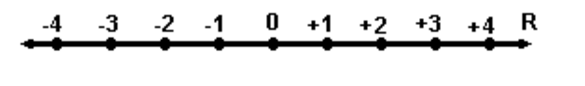
\includegraphics[width=4.39in,height=2.34in]{./media/image9.png}
	\end{Center}
\end{figure}


%%%%%%%%%%%%%%%%%%%% Figure/Image No: 9 Ends here %%%%%%%%%%%%%%%%%%%%

\par

\begin{adjustwidth}{0.69in}{0.0in}
\textbf{Figura 7.5} - Funções logarítmicas: variação do sinal dos coeficientes do antilogaritmo e do logaritmo.\par

\end{adjustwidth}


\vspace{\baselineskip}
{\fontsize{14pt}{16.8pt}\selectfont \textbf{EXERCÍCIOS 7}\par}\par


\vspace{\baselineskip}
\begin{enumerate}
	\item Faça os gráficos das funções usando uma tabela de valores de \textit{x} e \textit{y}. (use a calculadora para encontrar os logaritmos)\par

\begin{enumerate}
	\item \textit{F(x) = log x\tab }\tab c) \textit{G(x) = log (2x)}\par

	\item \textit{H(x) = 2 log x\tab }\tab d) \textit{J(x) = log (x\textsuperscript{2})}\par


\vspace{\baselineskip}
	\item a) Faça o gráfico das funções \textit{y = ln x}\ \ \ e\   \textit{y = e\textsuperscript{x}}.\  \par

b) Faça o gráfico da função \textit{y = x}.\par

	\item Verifique se existe simetria entre as funções \textit{y = ln x}\ \ \ e\   \textit{y = e\textsuperscript{x}}, em relação à função identidade\ \ \ \ \  \textit{y = x}.
\end{enumerate}\par


\vspace{\baselineskip}
	\item Faça um esboço do gráfico das funções logarítmicas sem usar a tabela.\par

\begin{enumerate}
	\item \textit{F(x) = ln (2x)} \tab \tab \tab c) \textit{Y(x) = -ln (3x)}\par

	\item \textit{P(x) = -log (-5x)\tab \tab \tab }d) \textit{Q(x) = 2 log (2x)} 
\end{enumerate}\par


\vspace{\baselineskip}
	\item Faça um esboço do gráfico e determine o domínio e a imagem das funções:\par

\begin{enumerate}
	\item \textit{F(x) = ln\ (x -  2) \tab \tab }\tab c) \textit{Y(x) = -ln (3+x)}\par

	\item \textit{P(x) = -ln (3- x)\tab \tab }\tab d) \textit{Q(x) = 2 log (x + 1)} 
\end{enumerate}\par


\vspace{\baselineskip}
	\item Utilize um aplicativo computacional para fazer o gráfico das funções. Determine o domínio e a imagem.\par

\begin{enumerate}
	\item \textit{F(x) = ln (x\textsuperscript{2}) \tab \tab }\tab c) \textit{Y(x) = ln (1-3x)}\par

	\item \textit{P(x) = log \textsuperscript{2}(x)\tab \tab \tab }d) \textit{Q(x) =\  log (x\textsuperscript{2} - 1)} 
\end{enumerate}\par


\vspace{\baselineskip}
	\item Calcule as raízes das funções:
\end{enumerate}\par

\begin{adjustwidth}{0.75in}{0.0in}
a) \textit{F(x) = log (2x -\  1) \tab }\tab c) \textit{Y(x) = -log (5 - x\textsuperscript{2})}\par

\end{adjustwidth}

\begin{adjustwidth}{0.75in}{0.0in}
b) \textit{P(x) = -ln (3- 6x)\tab \tab }\tab d) \textit{Q(x) = 2 log (-x + 1)}\par

\end{adjustwidth}

\begin{adjustwidth}{0.75in}{0.0in}
 \par

\end{adjustwidth}

\begin{adjustwidth}{0.3in}{0.0in}
\textbf{7.7}\  Faça um esboço do gráfico das funções manualmente e sem fazer tabela. Interprete as informações contidas nos coeficientes.\par

\end{adjustwidth}

\begin{enumerate}
	\item \textit{F(x) = ln x +2} \tab \tab c) \textit{Y(x) = ln x – 3 \tab }e)\textit{ R(x) = ln(-x) +1}\par

	\item \textit{P(x) = -log x +3\tab }\tab d) \textit{Q(x) = 2ln x + 1 \tab }f)\textit{ T(x) = ln(-2x) -2} 
\end{enumerate}\par


\vspace{\baselineskip}

\vspace{\baselineskip}
\begin{enumerate}
	\item {\fontsize{14pt}{16.8pt}\selectfont \textbf{Aplicações de funções exponenciais e logarítmicas}\par}
\end{enumerate}\par


\vspace{\baselineskip}
Os logaritmos, atualmente, são mais utilizados para resolução de equações exponenciais e como funções, do que para sua função original, dos tempos de Napier e Bürgi, de facilitar multiplicações e divisões de números muito pequenos ou muito grandes. Problemas de decaimento ou crescimento exponencial envolvem necessariamente o uso dos logaritmos.\par


\vspace{\baselineskip}
{\fontsize{14pt}{16.8pt}\selectfont \textbf{8.1 – Aplicações financeiras }\par}\par


\vspace{\baselineskip}
Considere-se uma aplicação financeira do tipo poupança, em que um capital inicial \textit{C\textsubscript{o }=\  R$\$$  1.000,00} é depositado no mês t = 0 e é corrigido mensalmente com uma taxa de juros constante de \textit{i = 0,5 $\%$ } do capital presente. O capital a cada mês pode ser calculado da seguinte maneira:\par


\vspace{\baselineskip}
\textit{C(1) = 1000 + 1000 $ \cdot $  (0,5/100) = 1000 $ \cdot $  (1+0,5/100) = 1000 $ \cdot $  1,005}\par


\vspace{\baselineskip}
\textit{C(2) = 1000 $ \cdot $  1,005 $ \cdot $  1,005 = 1000 $ \cdot $  1,005\textsuperscript{2}}\par


\vspace{\baselineskip}
\textit{C(3) = 1000 $ \cdot $  1,005\textsuperscript{2}\  $ \cdot $ \ 1,005 =  1000 $ \cdot $  1,005\textsuperscript{3}}\par


\vspace{\baselineskip}
Ou para este caso,\ \  \textit{C(t) = 1000 $ \cdot $  1,005\textsuperscript{t}} \ \ \  onde \textit{t} é o tempo em meses.\tab (8.1)\par


\vspace{\baselineskip}
Com a função (8.1) pode-se calcular o capital (montante) da poupança para qualquer tempo \textit{t}. Com essa função também pode-se calcular o tempo necessário para que a poupança atinja determinado capital \textit{C}, simplesmente resolvendo (8.1) para \textit{t}:\par


\vspace{\baselineskip}
\textit{C = 1000 $ \cdot $  1,005\textsuperscript{t}} . Dividindo por \textit{1000}, tem-se\par

 \( \frac{C}{1000}=1,005^{t} \) .\ \ \  Aplicando logaritmo natural em ambos os lados da equação, tem-se\par


\vspace{\baselineskip}
 \( ln\frac{C}{1000}=ln1,005^{t}~~~~ ^{} \) . Usando a propriedade da potência, tem-se\par


\vspace{\baselineskip}
 \( ln\frac{C}{1000}=t \cdot ln1,005^{}~~~~ ^{} \) . Isolando \textit{t}, tem-se\par


\vspace{\baselineskip}
  \( t=\frac{ln\frac{C}{1000}}{ln1,005}~  \) . ■\par


\vspace{\baselineskip}
\textbf{Exercícios 8.1}\par


\vspace{\baselineskip}
\begin{enumerate}
	\item Escreva a Eq. 8.1 na forma generalizada. Utilize\  \textit{C\textsubscript{o}} para expressar o capital inicial e\   \textit{j} \  para a taxa de juros, sendo\par

 \( j=1+\frac{i}{100} \) .\par


\vspace{\baselineskip}
	\item Calcule o capital de uma poupança sendo\  \textit{C\textsubscript{o}= R$\$$  500,00 },\textit{ i=0,45 }ao mês, depois de \textit{3 }anos.\ \  \par

	\item Calcule o tempo necessário de uma poupança, para que o capital atinja o valor de \textit{C =} \textit{R$\$$  20.000,00}, sendo\  \textit{C\textsubscript{o}=R$\$$  1.500,00 } e\textit{ i=0,6 }ao mês.\  \par

	\item Calcule\ a\ taxa de juros   \textit{j}\  e a taxa de rendimento mensal \textit{\  i } de uma aplicação tipo poupança em que \textit{C\textsubscript{o}=R$\$$  500,00},\ sendo\ que\ o\ capital\ inicial ficou aplicado durante 5 anos e chegou ao montante de R$\$$   2.500,00.     \par

	\item Um pai emprestou\  \textit{R$\$$  5.500,00} a seu filho, que demorou \textit{3} anos para pagar. Considerando a taxa de\textit{ i=0,6 }ao mês, qual é a dívida do filho?\ \  
\end{enumerate}\par


\vspace{\baselineskip}
{\fontsize{14pt}{16.8pt}\selectfont \textbf{8.2. Desvalorização de bens}\par}\par


\vspace{\baselineskip}
Alguns bens, tais como carros, apartamentos, casas, barcos e outros sofrem desvalorização com o passar do tempo. Se a cada ano o bem desvalorizasse sempre o mesmo valor teríamos uma taxa constante de desvalorização. Porém, não é o que ocorre na realidade. Na maioria dos casos essa desvalorização não é proporcional ao tempo, ou seja, a taxa de desvalorização não é constante. A Tabela 8.2.1 dá o preço de mercado de dois modelos de carro. \par


\vspace{\baselineskip}
Tabela 8.2.1 – Preços (em reais x 1000) de dois modelos de carro em função do tempo (em anos).\par



%%%%%%%%%%%%%%%%%%%% Table No: 3 starts here %%%%%%%%%%%%%%%%%%%%


\begin{table}[H]
 			\centering
\begin{tabular}{p{0.78in}p{0.55in}p{0.49in}p{0.49in}p{0.49in}p{0.49in}p{0.49in}p{0.49in}}
\hline
%row no:1
\multicolumn{1}{|p{0.78in}}{} & 
\multicolumn{1}{|p{0.55in}}{0} & 
\multicolumn{1}{|p{0.49in}}{1} & 
\multicolumn{1}{|p{0.49in}}{2} & 
\multicolumn{1}{|p{0.49in}}{3} & 
\multicolumn{1}{|p{0.49in}}{4} & 
\multicolumn{1}{|p{0.49in}}{5} & 
\multicolumn{1}{|p{0.49in}|}{6} \\
\hhline{--------}
%row no:2
\multicolumn{1}{|p{0.78in}}{Modelo 1 (R$\$$ x1000)} & 
\multicolumn{1}{|p{0.55in}}{49} & 
\multicolumn{1}{|p{0.49in}}{43} & 
\multicolumn{1}{|p{0.49in}}{35} & 
\multicolumn{1}{|p{0.49in}}{32} & 
\multicolumn{1}{|p{0.49in}}{30} & 
\multicolumn{1}{|p{0.49in}}{28} & 
\multicolumn{1}{|p{0.49in}|}{27} \\
\hhline{--------}
%row no:3
\multicolumn{1}{|p{0.78in}}{Modelo 2 (R$\$$ x1000)} & 
\multicolumn{1}{|p{0.55in}}{30} & 
\multicolumn{1}{|p{0.49in}}{25} & 
\multicolumn{1}{|p{0.49in}}{23} & 
\multicolumn{1}{|p{0.49in}}{22} & 
\multicolumn{1}{|p{0.49in}}{20,8} & 
\multicolumn{1}{|p{0.49in}}{20} & 
\multicolumn{1}{|p{0.49in}|}{19,5} \\
\hhline{--------}

\end{tabular}
 \end{table}


%%%%%%%%%%%%%%%%%%%% Table No: 3 ends here %%%%%%%%%%%%%%%%%%%%


\vspace{\baselineskip}
Podemos associar a desvalorização de cada modelo a um número e com ele tomar a decisão de compra. Consideremos a função exponencial como o modelo matemático da desvalorização dos carros.\par


\vspace{\baselineskip}
\textit{P(t) = P\textsubscript{o} $ \cdot $  e \textsuperscript{– kt}}{\fontsize{14pt}{16.8pt}\selectfont \textit{\ \ \ \  \tab \tab \tab \tab \tab \tab \tab }(8.2.1)\par}\par


\vspace{\baselineskip}
Onde \textit{P} é o preço (em R$\$$ x1000), \textit{P\textsubscript{o}\  }é o preço do carro novo, \textit{t} é o tempo (anos) e \textit{k} é a constante característica da depreciação, de cada modelo de carro. A depreciação será maior, quanto maior for o valor de \textit{k}. \par


\vspace{\baselineskip}
Para calcular o valor de \textit{k}, precisamos resolver a Eq. (8.2.1) para \textit{k}. Dividindo esta equação por \textit{P\textsubscript{o}}, temos:\par


\vspace{\baselineskip}
 \( \frac{P \left( t \right) }{P_{0}}=e^{-kt} \) .\  \par

Aplicando logaritmo natural em ambos os lados da equação e usando a propriedade P3 dos logaritmos, temos:\par


\vspace{\baselineskip}
 \( ln \left( \frac{P \left( t \right) }{P_{0}} \right) =-kt  \) . dividindo por (\textit{– t}) (para \textit{t $ \neq $  0}), temos:\par


\vspace{\baselineskip}
 \( k=-\frac{1}{t}ln \left( \frac{P \left( t \right) }{P_{0}} \right)  \) \tab \tab \tab \tab \tab \tab \tab (8.2.2)\par


\vspace{\baselineskip}

\vspace{\baselineskip}
Se aplicamos a Eq.(8.2.2) para cada ano, obteremos, para esse exemplo, seis valores de \textit{k}, cuja média chamaremos de \textit{k} médio (\textit{k\textsubscript{m}}). Para os dados da Tab. 8.2.1 obtivemos os seguinte valores:\par

\tab Modelo 1: \textit{k\textsubscript{m} = 0,12913}\par

\tab Modelo 2: \textit{k\textsubscript{m} = 0,1105}.\par

Portanto, o Modelo 2 tem depreciação menor que o Modelo 1.\par


\vspace{\baselineskip}
Levando \textit{k\textsubscript{m}} na Eq.(8.2.1) no lugar de \textit{k}, obtemos uma função que descreve a desvalorização do modelo em função do tempo (Eq. 7.2.3).\par


\vspace{\baselineskip}
 \( P \left( t \right) =P_{0}e^{-k_{m}t} \) \textit{.\tab \tab \tab \tab \tab \tab \tab }(8.2.3)\par


\vspace{\baselineskip}


%%%%%%%%%%%%%%%%%%%% Figure/Image No: 10 starts here %%%%%%%%%%%%%%%%%%%%

\begin{figure}[H]
	\begin{Center}
		\includegraphics[width=4.0in,height=2.32in]{./media/image10.png}
	\end{Center}
\end{figure}


%%%%%%%%%%%%%%%%%%%% Figure/Image No: 10 Ends here %%%%%%%%%%%%%%%%%%%%

\par

\textbf{Figura 8.2.1}– Depreciação de carros\par


\vspace{\baselineskip}
A Figura 8.2.1 apresenta os dados da Tab. 8.2.1 (pontos) e as curvas de depreciação (curvas ajustadas) obtidas com a Eq. 8.2.3 e os respectivos valores de \textit{k\textsubscript{m}}\  para os modelos 1 e 2.■\par


\vspace{\baselineskip}
\textbf{Exercícios 8.2}\par


\vspace{\baselineskip}
\begin{enumerate}
	\item Utilize a Eq. 8.2.3 para calcular o valor do carro Modelo 1 depois de 10 anos.\par

	\item Pesquise dados de preços médios de carro de seu interesse na Tabela Fipe, para ao menos, 5 anos. Repita os procedimentos do Exemplo 8.2 e calcule \textit{k\textsubscript{m}}. Faça um gráfico de Preço por tempo, para visualizar a curva de depreciação do carro.\par

	\item Um apartamento custava R$\$$  500.000,00 em 2000, R$\$$  450.000,00 em 2010 e R$\$$  400.000,00 em 2014. Determine o coeficiente de desvalorização\  \textit{k\textsubscript{m}\textsuperscript{ }}.
\end{enumerate}\par


\vspace{\baselineskip}

\vspace{\baselineskip}
{\fontsize{14pt}{16.8pt}\selectfont \textbf{8.3 – Linearização de gráficos de funções exponenciais}\par}\par


\vspace{\baselineskip}
Em algumas aplicações de funções exponenciais do tipo \par


\vspace{\baselineskip}
 \textit{y = f(x) = Ae\textsuperscript{kx}} , \par


\vspace{\baselineskip}
podemos\ escrever  \textit{f(x)} com uma reta, aplicando logaritmo natural nos dois lados da equação e usando a propriedade do produto, temos:\par


\vspace{\baselineskip}
\textit{ln y = ln A\ \ +\   ln e\textsuperscript{kx}}. Usando a propriedade P3 dos logaritmos, temos:\par


\vspace{\baselineskip}
\textit{ln y = ln A\  + kx\ .\   }Fazendo\textit{ Y = ln y\  }e\textit{\ \ b =  ln a, }temos:\par


\vspace{\baselineskip}
\textit{Y = b + kx.\tab \tab \tab \tab \tab \tab \tab \tab \tab }(8.3.1)\par


\vspace{\baselineskip}
A Eq. (8.31) é uma equação de reta, onde \textit{b} é o coeficiente linear e \textit{k} o angular. Com esta equação, o cálculo de \textit{k} ou de \textit{x} fica elementar:\par


\vspace{\baselineskip}
 \( k=\frac{1}{x} \left( Y-b \right)  \) \ \ \ \ \ \  e\ \ \   \( x=\frac{1}{k} \left( Y-b \right)  \) .\par


\vspace{\baselineskip}
\textbf{Exercícios 8.3}\par


\vspace{\baselineskip}
\begin{enumerate}
	\item Utilize a ideia de linearização das funções exponenciais para calcular \textit{k\textsubscript{m}} na equação de desvalorização de bens (Eq. 8.2.1).\par

	\item Utilize a ideia de linearização das funções exponenciais para calcular\  \textit{t }na equação de desvalorização de bens (Eq. 8.2.1).\par

	\item Se uma população de bactérias decresce, em um determinado período, de acordo com a função \textit{P(t) = 100e\textsuperscript{-0,5t}}, onde \textit{P} é o número de indivíduos e t é o tempo em minutos:
\end{enumerate}\par

\begin{enumerate}
	\item Aplique logaritmo na expressão da função, para escrevê-la na forma da Eq. 8.3.1. Determine os coeficientes angular e linear.\par

	\item Calcule o tempo em que a população será 1/3 da população inicial (100 indivíduos).\par

	\item Faça o gráfico das funções \textit{P(t)} e da função linearizada obtida no ítem\ (a).  
\end{enumerate}\par


\vspace{\baselineskip}
{\fontsize{14pt}{16.8pt}\selectfont \textbf{8.4 - Crescimento ou decrescimento populacional}\par}\par


\vspace{\baselineskip}
{\fontsize{14pt}{16.8pt}\selectfont \textbf{8.4.1 – Crescimento de bactérias }\par}\par

A quantidade de bactérias que se reproduzem por mitose (cada ser se divide em dois seres idênticos), considerando que não haja morte de indivíduos, pode ser modelada da seguinte maneira: \par


\vspace{\baselineskip}
Geração\  zero :\ 1 bactéria  \par

1ª geração :\ 2 bactéria  ; \textit{P = 2\textsuperscript{1}}\par

2ª geração : 4 bactéria ; \textit{P = 2\textsuperscript{2}}\par

3ª geração : 8 bactéria ; \textit{P = 2\textsuperscript{3}}\par

4ª geração : 16 bactéria;\  \textit{P = 2\textsuperscript{4}}\par

5ª geração : 32 bactéria;\  \textit{P = 2\textsuperscript{5}}\par


\vspace{\baselineskip}
A função\textit{\ \  P(n) = 2\textsuperscript{n}\ \  \tab \tab \tab \tab \tab \tab \tab \tab }(8.4.1)\par


\vspace{\baselineskip}

\vspace{\baselineskip}
onde \textit{P} é o número de bactérias e \textit{n }é a geração, permite calcular a população para qualquer tempo, desde que se saiba o tempo \textit{t} necessário para a reprodução de uma geração. Por exemplo, se \textit{n = 5}\  e \textit{t = 2 h}, em \textit{10} horas a população é \textit{32} bactérias. \par


\vspace{\baselineskip}
Se precisamos saber em quanto tempo a população atingirá 5000 indivíduos, aplicamos logaritmo de base \textit{2} na Eq. 8.4.1 e temos :\par


\vspace{\baselineskip}
 \( log_{2}P=log_{2}2^{n} \) . Utilizando a propriedade P3 dos logaritmos, temos:\par


\vspace{\baselineskip}
 \( n=log_{2}P \) . Usando \textit{P = 5000}, temos:\par


\vspace{\baselineskip}
 \( n=log_{2}5000 \)  . Escrevendo este logaritmo na base e, temos:\par


\vspace{\baselineskip}
 \( n=\frac{ln5000}{ln2}=12,28 \)  gerações. Ou, aproximadamente \textit{12} gerações, o que significa \textit{24 h}.\par

 \par


\vspace{\baselineskip}
{\fontsize{14pt}{16.8pt}\selectfont \textbf{8.4.2 – Decaimento bacteriano}\par}\par


\vspace{\baselineskip}
As bactérias que vivem no organismo humano, quando colocadas na água ou no solo, não sobrevivem por muito tempo. Assim, a população de bactérias presentes nos esgotos tende a diminuir. O fenômeno é conhecido como $``$decaimento bacteriano$"$  e é modelado pela função \par


\vspace{\baselineskip}
\textit{P(t) = P\textsubscript{o} $ \cdot $  e \textsuperscript{– kt}}{\fontsize{14pt}{16.8pt}\selectfont \textit{\ \ \ \  \tab \tab \tab \tab \tab \tab \tab }(8.4.2)\par}\par


\vspace{\baselineskip}
Onde \textit{P} é a população (número de indivíduos), \textit{P\textsubscript{o}\  }é a população inicial, \textit{t} é o tempo (horas) e \textit{k} é a constante ou taxa característica do decaimento, a qual depende de vários fatores, dentre eles o tipo de bactéria, a temperatura e a acidez do ambiente. O decaimento será maior, quanto maior for o valor de \textit{k}. \par


\vspace{\baselineskip}
Geralmente, o interesse de um pesquisador é determinar o tempo necessário para que metade da população seja exterminada. Esse tempo é conhecido como \textit{meia vida}. Na meia vida a população é \textit{P = P\textsubscript{o}/2}. Substituindo esse valor de P na Eq. 8.4.2, temos:\par


\vspace{\baselineskip}
\textit{ P\textsubscript{o}/2= P\textsubscript{o} $ \cdot $  e \textsuperscript{– kt}}{\fontsize{14pt}{16.8pt}\selectfont \textit{\  \  . }Cancelando\textit{ P\textsubscript{o} .}\par}\par


\vspace{\baselineskip}
\begin{adjustwidth}{1.57in}{0.0in}
 \( \frac{1}{2}=e^{-kt} \) {\fontsize{14pt}{16.8pt}\selectfont \textit{. }Aplicando logaritmo natural nos dois lados da equação e isolando \textit{t}, temos\textit{ }\par}\par

\end{adjustwidth}

{\fontsize{14pt}{16.8pt}\selectfont \textit{ }\par}\par

 \( t=-\frac{1}{k}~~ ln  \left( \frac{ 1}{2} \right)  \) {\fontsize{14pt}{16.8pt}\selectfont \  que é a meia vida.\par}\par


\vspace{\baselineskip}
\textbf{Exercícios 8.4}\par

\begin{enumerate}
	\item Uma população de bactérias se reproduz em função do tempo de acordo com a função  \textit{P(t) = 2\textsuperscript{t} :}\par

\begin{enumerate}
	\item Calcule o número de bactérias depois de \textit{100s}. \par

	\item Em quanto tempo a população será de \textit{500} indivíduos.
\end{enumerate}\par

	\item Calcule a taxa \textit{k} de decaimento (Eq. 8.4.2), sendo que em \textit{80} s a população se reduziu à metade da população inicial.\par

	\item Em um tempo \textit{t = 0 h} a população de bactérias era de \textit{1000000} de indivíduos. Passadas \textit{6 h} a população se reduziu à metade da população inicial. Qual será a população quando \textit{t = 9 h} ?\par

	\item Sabendo que a meia vida de uma população é de \textit{3 h}:
\end{enumerate}\par

\begin{enumerate}
	\item Qual é o valor da taxa de decaimento \textit{k} ?\par

	\item Em quanto tempo a população se reduzirá a \textit{P\textsubscript{o}/4} ?\par


\vspace{\baselineskip}

\vspace{\baselineskip}

\vspace{\baselineskip}

\vspace{\baselineskip}
{\fontsize{14pt}{16.8pt}\selectfont \textbf{8.5 - Concentração de medicamentos no organismo humano}\par}\par


\vspace{\baselineskip}
\begin{justify}
Quando um medicamento é ingerido a corrente sanguínea o distribui por todo o organismo. Consideremos que a concentração (massa, em gramas, por unidade de volume de sangue) é a mesma em cada parte do corpo. A eliminação do medicamento ocorre na medida que o sangue vai passando pelos rins. Portanto, uma função concentração (C(t)) é decrescente, e tem um valor máximo inicial C\textsubscript{o}. Supondo que a variação da concentração seja uma função da massa medicamento presente no organismo, podemos propor um modelo exponencial, com a seguinte função:
\end{justify}\par

\begin{FlushRight}
 \( C \left( t \right) =C_{o}e^{at} \) \tab \tab \tab \tab \tab \tab (8.5.1)
\end{FlushRight}\par

\begin{justify}
Onde \textit{C} é a concentração do medicamento (\textit{g}), \textit{C\textsubscript{o}} é a dose inicial, \textit{t} é o tempo e \textit{a} uma constante real, sendo \textit{a < 0}.
\end{justify}\par

\begin{justify}
O tempo de meia-vida, ou simplesmente a meia-vida\  ($ \tau$ )\ é\ o tempo necessário para que metade da quantidade inicial   \textit{C\textsubscript{o}} seja eliminada. É comum usar a ideia de meia-vida para investigar a variação da concentração de medicamentos no sangue. Assim, fazendo \textit{C}($ \tau$ ) \textit{= C\textsubscript{o}/2} e substituindo em (8.5.1), temos:
\end{justify}\par

\begin{FlushRight}
 \( \frac{C_{o}}{2}=C_{o}e^{a \tau} \) \tab \tab \tab \tab \tab \tab (8.5.2)
\end{FlushRight}\par

\begin{justify}
Cancelando \textit{C\textsubscript{o}} , aplicando logaritmo natural em ambos os membros de (8.5.2) e resolvendo para $ \tau$ , temos uma expressão para o tempo de meia-vida:
\end{justify}\par

\begin{FlushRight}
 \(  \tau=-\frac{1}{a}ln2 \) \tab \tab \tab \tab \tab \tab (8.5.3)
\end{FlushRight}\par

\begin{justify}
Se a meia-vida do medicamento é conhecida, podemos resolver a Eq. (8.5.3) para \textit{a}. 
\end{justify}\par

\begin{FlushRight}
 \( a=-\frac{1}{ \tau}ln2 \) \tab \tab \tab \tab \tab \tab (8.5.4)
\end{FlushRight}\par


\vspace{\baselineskip}
\begin{justify}
{\fontsize{14pt}{16.8pt}\selectfont \textbf{8.5.1 – Concentração do medicamento: dose única}\par}
\end{justify}\par

\begin{justify}
Consideremos um medicamento cuja meia-vida é \textit{$ \tau$  = 4 h} e a dose \textit{C\textsubscript{o} = 800 mg}. Com a Eq.(4) podemos calcular \textit{a}, obtendo \textit{a = -0,17329}. Substituindo estes dados na Eq. (8.5.1), temos uma função que dá valores da concentração para cada instante de tempo, da dose inicial.
\end{justify}\par

\begin{FlushRight}
 \( C \left( t \right) =800e^{-0,17329 t} \) \tab \tab \tab \tab (8.5.5)
\end{FlushRight}\par

\begin{justify}
A Fig. 1 apresenta os valores da concentração obtidos com a função da Eq.(5), onde pode-se verificar que o tempo para a eliminação da metade da dose inicial (meia-vida) é \textit{4 h} e que em torno de \textit{40h} a concentração é mínima, para estes dados. É importante observar que a posição da curva depende da meia-vida do medicamento, que é, em resumo, um ponto da curva onde \textit{C = C\textsubscript{o}/2} e que caracteriza o comportamento do medicamento no organismo. 
\end{justify}\par


\vspace{\baselineskip}


%%%%%%%%%%%%%%%%%%%% Figure/Image No: 11 starts here %%%%%%%%%%%%%%%%%%%%

\begin{figure}[H]
	\begin{Center}
		\includegraphics[width=5.01in,height=3.01in]{./media/image11.jpeg}
	\end{Center}
\end{figure}


%%%%%%%%%%%%%%%%%%%% Figure/Image No: 11 Ends here %%%%%%%%%%%%%%%%%%%%

\par

Figura 8.5.1 – Concentração de uma dose de medicamento: \textit{C\textsubscript{o} = 800}, \textit{a = -0,17329} \ \ \  e \textit{$ \tau$  = 4 h}. \par


\vspace{\baselineskip}
\begin{justify}
{\fontsize{14pt}{16.8pt}\selectfont \textbf{8.5.2 – Concentração do medicamento: doses múltiplas}\par}
\end{justify}\par

\begin{justify}
Consideremos que um paciente tenha ingerido o medicamento de 8 em 8h (intervalo de tempo de ingestão) e que cada dose seja eliminada com a mesma meia-vida. Para calcular a concentração total em função do tempo, devemos calcular a concentração de cada dose independentemente, utilizando a Eq.(8.5.1). Somando as concentrações em tempo de ingestão, obtemos a concentração de todas as doses em função do tempo. A Tab. 1 apresenta este método e foi obtida com os mesmos dados do item \textbf{8.5.1} (dose única). 
\end{justify}\par

\begin{justify}
Observando as somas (Total) em função do tempo, percebemos elas tendem a um valor específico, que é o limite da concentração do medicamento no organismo. Esse efeito pode ser observado claramente na Fig.8.5.2.
\end{justify}\par


\vspace{\baselineskip}
\begin{justify}
\textbf{Tabela 8.5.1} – Concentração do medicamento para múltiplas doses
\end{justify}\par



%%%%%%%%%%%%%%%%%%%% Table No: 4 starts here %%%%%%%%%%%%%%%%%%%%


\begin{table}[H]
 			\centering
\begin{tabular}{p{0.47in}p{0.47in}p{0.47in}p{0.47in}p{0.47in}p{0.52in}p{0.52in}p{0.52in}p{0.52in}}
\hline
%row no:1
\multicolumn{1}{|p{0.47in}}{\multirowcell{2}{}{\begin{tabular}{p{0.47in}}Doses\\\end{tabular}}} & 
\multicolumn{8}{|p{5.18in}|}{\Centering Tempo (h)} \\
\hhline{~--------}
%row no:2
\multicolumn{1}{|p{0.47in}}{} & 
\multicolumn{1}{|p{0.47in}}{0} & 
\multicolumn{1}{|p{0.47in}}{8} & 
\multicolumn{1}{|p{0.47in}}{16} & 
\multicolumn{1}{|p{0.47in}}{24} & 
\multicolumn{1}{|p{0.52in}}{32} & 
\multicolumn{1}{|p{0.52in}}{40} & 
\multicolumn{1}{|p{0.52in}}{48} & 
\multicolumn{1}{|p{0.52in}|}{56} \\
\hhline{---------}
%row no:3
\multicolumn{1}{|p{0.47in}}{1} & 
\multicolumn{1}{|p{0.47in}}{400} & 
\multicolumn{1}{|p{0.47in}}{100} & 
\multicolumn{1}{|p{0.47in}}{25} & 
\multicolumn{1}{|p{0.47in}}{6,25} & 
\multicolumn{1}{|p{0.52in}}{1,5625} & 
\multicolumn{1}{|p{0.52in}}{0,390625} & 
\multicolumn{1}{|p{0.52in}}{0,097656} & 
\multicolumn{1}{|p{0.52in}|}{0,024414} \\
\hhline{---------}
%row no:4
\multicolumn{1}{|p{0.47in}}{2} & 
\multicolumn{1}{|p{0.47in}}{} & 
\multicolumn{1}{|p{0.47in}}{400} & 
\multicolumn{1}{|p{0.47in}}{100} & 
\multicolumn{1}{|p{0.47in}}{25} & 
\multicolumn{1}{|p{0.52in}}{6,25} & 
\multicolumn{1}{|p{0.52in}}{1,5625} & 
\multicolumn{1}{|p{0.52in}}{0,390625} & 
\multicolumn{1}{|p{0.52in}|}{0,097656} \\
\hhline{---------}
%row no:5
\multicolumn{1}{|p{0.47in}}{3} & 
\multicolumn{1}{|p{0.47in}}{} & 
\multicolumn{1}{|p{0.47in}}{} & 
\multicolumn{1}{|p{0.47in}}{400} & 
\multicolumn{1}{|p{0.47in}}{100} & 
\multicolumn{1}{|p{0.52in}}{25} & 
\multicolumn{1}{|p{0.52in}}{6,25} & 
\multicolumn{1}{|p{0.52in}}{1,5625} & 
\multicolumn{1}{|p{0.52in}|}{0,390625} \\
\hhline{---------}
%row no:6
\multicolumn{1}{|p{0.47in}}{4} & 
\multicolumn{1}{|p{0.47in}}{} & 
\multicolumn{1}{|p{0.47in}}{} & 
\multicolumn{1}{|p{0.47in}}{} & 
\multicolumn{1}{|p{0.47in}}{400} & 
\multicolumn{1}{|p{0.52in}}{100} & 
\multicolumn{1}{|p{0.52in}}{25} & 
\multicolumn{1}{|p{0.52in}}{6,25} & 
\multicolumn{1}{|p{0.52in}|}{1,5625} \\
\hhline{---------}
%row no:7
\multicolumn{1}{|p{0.47in}}{5} & 
\multicolumn{1}{|p{0.47in}}{} & 
\multicolumn{1}{|p{0.47in}}{} & 
\multicolumn{1}{|p{0.47in}}{} & 
\multicolumn{1}{|p{0.47in}}{} & 
\multicolumn{1}{|p{0.52in}}{400} & 
\multicolumn{1}{|p{0.52in}}{100} & 
\multicolumn{1}{|p{0.52in}}{25} & 
\multicolumn{1}{|p{0.52in}|}{6,25} \\
\hhline{---------}
%row no:8
\multicolumn{1}{|p{0.47in}}{6} & 
\multicolumn{1}{|p{0.47in}}{} & 
\multicolumn{1}{|p{0.47in}}{} & 
\multicolumn{1}{|p{0.47in}}{} & 
\multicolumn{1}{|p{0.47in}}{} & 
\multicolumn{1}{|p{0.52in}}{} & 
\multicolumn{1}{|p{0.52in}}{400} & 
\multicolumn{1}{|p{0.52in}}{100} & 
\multicolumn{1}{|p{0.52in}|}{25} \\
\hhline{---------}
%row no:9
\multicolumn{1}{|p{0.47in}}{7} & 
\multicolumn{1}{|p{0.47in}}{} & 
\multicolumn{1}{|p{0.47in}}{} & 
\multicolumn{1}{|p{0.47in}}{} & 
\multicolumn{1}{|p{0.47in}}{} & 
\multicolumn{1}{|p{0.52in}}{} & 
\multicolumn{1}{|p{0.52in}}{} & 
\multicolumn{1}{|p{0.52in}}{400} & 
\multicolumn{1}{|p{0.52in}|}{100} \\
\hhline{---------}
%row no:10
\multicolumn{1}{|p{0.47in}}{8} & 
\multicolumn{1}{|p{0.47in}}{} & 
\multicolumn{1}{|p{0.47in}}{} & 
\multicolumn{1}{|p{0.47in}}{} & 
\multicolumn{1}{|p{0.47in}}{} & 
\multicolumn{1}{|p{0.52in}}{} & 
\multicolumn{1}{|p{0.52in}}{} & 
\multicolumn{1}{|p{0.52in}}{} & 
\multicolumn{1}{|p{0.52in}|}{400} \\
\hhline{---------}
%row no:11
\multicolumn{1}{|p{0.47in}}{TOTAL} & 
\multicolumn{1}{|p{0.47in}}{400} & 
\multicolumn{1}{|p{0.47in}}{500} & 
\multicolumn{1}{|p{0.47in}}{525} & 
\multicolumn{1}{|p{0.47in}}{531,25} & 
\multicolumn{1}{|p{0.52in}}{532,8125} & 
\multicolumn{1}{|p{0.52in}}{533,2031} & 
\multicolumn{1}{|p{0.52in}}{533,3008} & 
\multicolumn{1}{|p{0.52in}|}{533,3252} \\
\hhline{---------}

\end{tabular}
 \end{table}


%%%%%%%%%%%%%%%%%%%% Table No: 4 ends here %%%%%%%%%%%%%%%%%%%%


\vspace{\baselineskip}


%%%%%%%%%%%%%%%%%%%% Figure/Image No: 12 starts here %%%%%%%%%%%%%%%%%%%%

\begin{figure}[H]
	\begin{Center}
		\includegraphics[width=5.01in,height=3.01in]{./media/image12.jpeg}
	\end{Center}
\end{figure}


%%%%%%%%%%%%%%%%%%%% Figure/Image No: 12 Ends here %%%%%%%%%%%%%%%%%%%%

\par

\begin{justify}
Figura 8.5.2 – Concentração acumulada de várias doses: \textit{C\textsubscript{o} = 800}, \textit{a = -0,17329} ,\  \textit{$ \tau$  = 4 h} e tempo de ingestão de \textit{8 h}.
\end{justify}\par

\begin{justify}
\textbf{Exercícios 8.5:}
\end{justify}\par

\begin{justify}
\textbf{8.5.1}  Utilizando as Eqs. (8.5.1) a (8.5.3) e uma tabela eletrônica, calcule as concentrações de um medicamento ingerido em dose única para um período de \textit{48 h}, com \textit{C\textsubscript{o} = 500mg/cm\textsuperscript{3}}\ \  com os seguintes tempos de meia-vida: (apresente os resultados em um mesmo gráfico)
\end{justify}\par

\begin{justify}
a)\  \textit{$ \tau$ \  = 5 h} \tab \tab b)\  \textit{$ \tau$ \  = 8 h\  \tab \ \ \  }c)\  \textit{$ \tau$ \  = 10 h\  \tab }d)\  \textit{$ \tau$ \  = 12 h\  }
\end{justify}\par

\begin{justify}
\textbf{8.5.2 }Desenvolva uma tabela eletrônica semelhante à Tab. 8.5.1, de maneira que a meia-vida, a dose inicial e o tempo de ingestão sejam manipuláveis pelo usuário. Calcule a concentração de medicamentos para os seguintes dados:
\end{justify}\par

\begin{justify}
a) Dados \textit{$ \tau$ \  = 4 h\  }e \textit{C\textsubscript{o} = 800mg/cm\textsuperscript{3 }}, determine o intervalo de ingestão para que a concentração máxima seja próxima de \textit{1000} \textit{mg/cm\textsuperscript{3}}\ .\ \ \   
\end{justify}\par

\begin{justify}
b) Dados \textit{$ \tau$ \  = 4 h\  }e \textit{C\textsubscript{o} = 800mg/cm\textsuperscript{3}}, determine o intervalo de ingestão para a concentração máxima fique próxima de \textit{915 mg/cm\textsuperscript{3}} .
\end{justify}\par


\vspace{\baselineskip}
\textbf{BIBLIOGRAFIA}\par

ANTON, H; BIVENS, I. e DAVIS, S. \textit{Cálculo}. Porto Alegre: Bookmann, 2007.\par

\setlength{\parskip}{0.0pt}
FEITOSA, Ailton. \textbf{Aplicação dos Logaritmos. }Disponível em: <http://www.infoescola.com/matematica/aplicacoes-dos-logaritmos/>. Acesso em: 02 nov. 2014.\par

\setlength{\parskip}{8.04pt}
FLORIANI, J. V. \textit{Função Logarítmica}. (Coleção Arithmos) Blumenau: Ed. Da FURB, 1999.\par

GENTIL, N.; SANTOS, C.A.M.; GRECCO, A.C; BELLOTTO FILHO, A. e GRECCO, S.E. \textit{Matemática para o 2º Grau}. São Paulo: Ed. Ática S.A, 1990.\par

\setlength{\parskip}{0.0pt}
IEZZI, Gelson; DOLCE, Osvaldo; MURAKAMI, Carlos.\textbf{ Fundamentos de matemática elementar, 2: logaritmos.} 9. ed. São Paulo: Atual, 2004.\par

\setlength{\parskip}{8.04pt}
LIMA, E. L. \textit{Logaritmos} (Coleção Fundamentos da Matemática Elementar). Brasília: Sociedade Brasileira de Matemática. 1980.\par

\setlength{\parskip}{0.0pt}
SÁ, Robison. \textbf{História dos logaritmos. }Disponível em: <http://www.infoescola.com/matematica/historia-dos-logaritmos/>. Acesso em: 06 nov. 2014.\par

SILVA, Marcos Noé Pedro da. \textbf{Logaritmos. }Disponível em: http://www.mundoeducacao.com/matematica/logaritmos.htm>.\  Acesso em: 07 nov. 2014.\par

SILVA, Marcos Noé Pedro da. \textbf{Aplicação dos logaritmos. }Disponível em: < http://www.mundoeducacao.com/matematica/aplicacao-dos-logaritmos.htm\par

>. Acesso em: 21 nov. 2014.\par


\vspace{\baselineskip}
\setlength{\parskip}{8.04pt}

\vspace{\baselineskip}
\textbf{RESPOSTAS DOS EXERCÍCIOS}\par


\vspace{\baselineskip}

\vspace{\baselineskip}
\textbf{EXERCÍCIOS 2}\par

\textbf{2.1 \tab }a) 3\tab \tab b) 6\tab \tab c) 3/2\tab \tab d) -3 \tab \tab e) 2\tab \tab f) -5/2\par

\textbf{2.2\tab }a) 5\tab \tab b) -4\tab \tab c) -2\tab \tab d) 3\tab \tab e) 5\tab \tab f) ¼\par

\ \  \tab g) -5\tab \tab h) -2/3\tab \tab i) -1/2\par

\textbf{2.3 \tab }a) 81\tab \tab b) 2\tab \tab c)  \( \sqrt[125]{5} \) \tab d)  \( 2+2\sqrt[]{2} \) \tab e) -2\tab \tab f) 2\par

\textbf{2.4\tab }Não faz sentido calcular um logaritmo de base 1, pois ao aplicar a definição teremos 1\textsuperscript{n}= x, e independente de \textit{n} será encontrado x = 1, devido a uma propriedade das potências onde 1\textsuperscript{n }= 1.\par

\textbf{2.5\tab }Não faz sentido calcular um logaritmo com base negativa pois em determinadas equações não será possível encontrar um número que satisfaça a identidade.\par

\textbf{2.6\tab }Não faz sentido calcular o logaritmo de um número negativo, pois nem sempre será possível encontrar uma solução que pertença aos números reais.\par

\textbf{2.7 }\tab 0 < x < 1\par

\textbf{2.8\tab }a) x > 2\tab b) x > ¼\tab c) x > ½ e x $ \neq $  1\tab d) x > 4\par


\vspace{\baselineskip}
\textbf{EXERCÍCIOS 3}\par

\textbf{3.1}\tab a) -3\tab \tab b) -4\tab \tab c) 11\tab \tab d) ¼\par

\textbf{3.2}\tab a) 16\tab \tab b) 40\tab \tab c) 3\tab \tab d) 2\tab \tab e) 3\tab f) 625/2\par

\textbf{3.3\ \ \ \ \  }Pela propriedade P7 temos que  \(  \left( -1 \right) log_{a}y=log_{a}y^{-1} \) {\fontsize{14pt}{16.8pt}\selectfont . Usando P4,\ temos  \par}\par

{\fontsize{14pt}{16.8pt}\selectfont =  \( a^{log_{a} \left( y \right) ^{-1}}=y^{-1}=\frac{1}{y} \) .\par}\par

\textbf{3.4 }\tab a) ln 3\tab = 1,0986...\tab b) 2/5\tab \tab c)  \( \sqrt[]{ln600} \)  = 2,5292....\tab d)\   \( \sqrt[]{1+ln\frac{2}{3}} \) \par

\textbf{3.5 \tab  \( \frac{25}{9} \) }{\fontsize{14pt}{16.8pt}\selectfont  \par}\par

\textbf{3.6} a) V = 1,411 x 10\textsuperscript{18\ \  }\ \ \ \ \  b) V = 1,411 x 10\textsuperscript{18}\par


\vspace{\baselineskip}
\textbf{EXERCÍCIOS 4}\par

\textbf{4.1 }\tab a) 1\tab \tab b) 5 \tab \tab c) 3\tab \tab d) 10\tab \tab e) -5\tab \tab f) -3\tab \par

\textbf{4.2}\tab a) 0,3010...\tab b) 1,9459...\tab c) 1,3010...\tab d) 1,8450...\tab e) 2,8903...\tab f) 4\par

\tab g) 1\tab \tab h) 0\par

\textbf{4.3}\tab a) 1,5849...\tab b) 0,4306...\tab c) 1,4306...\tab d) 1,6094...\par

\textbf{4.4\tab }a) 1,5849...\tab b) 0,4306...\tab c) 1,4306...\tab d) 0,6989...\par

\textbf{4.5\tab }a)  \( \frac{log_{}2}{log_{}e} \) \tab b)  \( \frac{log_{}20}{log_{}e} \) \tab c)  \( \frac{log_{}18}{log_{}e} \) \tab d)  \( \frac{log_{}e}{log_{}e}=1 \) {\fontsize{14pt}{16.8pt}\selectfont  \par}\par

\textbf{4.6 \tab }a)  \( \frac{ln25}{ln10} \) \tab \tab b)  \( \frac{ln7}{ln10} \) \tab \tab c)  \( \frac{-ln5}{ln10} \) \tab \tab d)  \( \frac{ln3-ln4}{ln10} \) \par

\textbf{4.7 }\tab - 0,1249... = (0,4771...) – (0,6020) = - 0,1249...\par


\vspace{\baselineskip}
\setlength{\parskip}{6.0pt}
\textbf{EXERCÍCIOS 5}\par

\begin{enumerate}[label*={\fontsize{12pt}{12pt}\selectfont \textbf{\arabic*.}}]
	\item a) 2\tab \tab b) 1\tab \tab c) 1\tab \tab d) S=$ \{ $  \( \sqrt[]{10},100 \) $ \} $ 
\end{enumerate}\par

\textbf{5.2} a)  \( \frac{log10}{log2} \) \tab b)  \( \sqrt[]{\frac{ln100}{2}} \) \tab c)  \( -\frac{2}{3} \) \tab \ \ \ \  d)  \( \frac{log2}{4} \) \tab e) S=$ \{ $ 1,3$ \} $ \tab f) 4 \textbf{+} log 2\par

\textbf{5.3\tab }a) -2\tab \tab b) 2\tab \tab c) S=$ \{ $ -2,0$ \} $ \tab d)  \( \frac{3}{8} \) \par

\textbf{5.4}\tab É possível resolver usando a definição de logaritmo.\par

\textbf{5.5\tab }a) 2\tab \tab b) S=$ \{ $ -1,3$ \} $ \tab c)  \( \frac{1}{2} \) \tab \par

\textbf{5.6 \tab }É possível resolver usando a definição de logaritmo.\par

\textbf{5.7\tab }a) 100\tab \ \ \  b) 10\textsuperscript{5\tab }c)  \( \sqrt[]{\frac{3}{100}} \) \tab d)  \( \frac{3}{10^{5}} \) \tab \tab e)  \( \frac{23}{3} \) \tab \tab f) S=$ \{ $ 1,9$ \} $ \par

\textbf{5.8\tab }a) 8\tab \tab b) 10/ln4\tab c)  \( \sqrt[3]{3} \) \tab \tab d) ln²4\par

\textbf{5.9\tab }Aproximadamente 381 meses.\par

\textbf{5.10\tab  \( t= \frac{log\frac{C}{C0}}{log⁡ \left( 1+\frac{i}{100} \right) } \) }\par

\textbf{5.11\tab  \( t= -\frac{1}{k}ln \left( \frac{1}{2} \right)  \) }\par

\textbf{5.12\tab }a) (usar \textit{u = log x});\  \textit{x\textsubscript{1} = 100}\ \ e  \textit{x\textsubscript{2} = 0,1}\ \ \ \ \ \ \ \ \  b) 9\tab \tab c)  \( \sqrt[]{2} \) \tab \tab d)  \( \sqrt[]{10} \) \par


\vspace{\baselineskip}
\setlength{\parskip}{8.04pt}

\vspace{\baselineskip}
\setlength{\parskip}{6.0pt}
\textbf{EXERCÍCIOS 6}\par


\vspace{\baselineskip}
\setlength{\parskip}{0.0pt}
\begin{enumerate}
	\item \tab a) f(g(x)) = 9x²-6x+1 ; g(f(x)) = 3x²-1\tab b) f(g(x)) = x ; g(f(x)) = x\par


\vspace{\baselineskip}
\tab c) f(g(x)) = x ; g(f(x)) = x\tab \tab \tab d) f(g(x)) = x ; g(f(x)) = x\par


\vspace{\baselineskip}
	\item a,b,d são funções inversas; c não é inversa\par


\vspace{\baselineskip}

\vspace{\baselineskip}

\end{enumerate}	\item a) \par



%%%%%%%%%%%%%%%%%%%% Figure/Image No: 13 starts here %%%%%%%%%%%%%%%%%%%%

\begin{figure}[H]
	\begin{Center}
		\includegraphics[width=2.91in,height=2.23in]{./media/image13.png}
	\end{Center}
\end{figure}


%%%%%%%%%%%%%%%%%%%% Figure/Image No: 13 Ends here %%%%%%%%%%%%%%%%%%%%

\par


\vspace{\baselineskip}

\vspace{\baselineskip}

\vspace{\baselineskip}

\vspace{\baselineskip}
b)\par



%%%%%%%%%%%%%%%%%%%% Figure/Image No: 14 starts here %%%%%%%%%%%%%%%%%%%%

\begin{figure}[H]
	\begin{Center}
		\includegraphics[width=2.77in,height=2.31in]{./media/image14.png}
	\end{Center}
\end{figure}


%%%%%%%%%%%%%%%%%%%% Figure/Image No: 14 Ends here %%%%%%%%%%%%%%%%%%%%

\par


\vspace{\baselineskip}

\vspace{\baselineskip}

\vspace{\baselineskip}

\vspace{\baselineskip}
	\item \tab \tab 
\vspace{\baselineskip}

%%%%%%%%%%%%%%%%%%%% Figure/Image No: 15 starts here %%%%%%%%%%%%%%%%%%%%

\begin{figure}[H]
	\begin{Center}
		\includegraphics[width=2.9in,height=2.26in]{./media/image15.png}
	\end{Center}
\end{figure}


%%%%%%%%%%%%%%%%%%%% Figure/Image No: 15 Ends here %%%%%%%%%%%%%%%%%%%%

\par



%%%%%%%%%%%%%%%%%%%% Figure/Image No: 16 starts here %%%%%%%%%%%%%%%%%%%%

\begin{figure}[H]
	\begin{Center}
		\includegraphics[width=2.91in,height=2.24in]{./media/image16.png}
	\end{Center}
\end{figure}


%%%%%%%%%%%%%%%%%%%% Figure/Image No: 16 Ends here %%%%%%%%%%%%%%%%%%%%

	\item  
\end{enumerate}\par

\begin{multicols}{2}

\vspace{\baselineskip}

\vspace{\baselineskip}

\end{multicols}
	\item a)  \( \sqrt[]{x-3} \) \tab b) x\textsuperscript{4}-2\tab \tab c) ln (x/5) – 2\tab d) 10\par


\vspace{\baselineskip}
\begin{enumerate}
	\item a) \par



%%%%%%%%%%%%%%%%%%%% Figure/Image No: 17 starts here %%%%%%%%%%%%%%%%%%%%

\begin{figure}[H]
	\begin{Center}
		\includegraphics[width=2.95in,height=2.68in]{./media/image17.png}
	\end{Center}
\end{figure}


%%%%%%%%%%%%%%%%%%%% Figure/Image No: 17 Ends here %%%%%%%%%%%%%%%%%%%%

\par

b)\par



%%%%%%%%%%%%%%%%%%%% Figure/Image No: 18 starts here %%%%%%%%%%%%%%%%%%%%

\begin{figure}[H]
	\begin{Center}
		\includegraphics[width=2.76in,height=2.57in]{./media/image18.png}
	\end{Center}
\end{figure}


%%%%%%%%%%%%%%%%%%%% Figure/Image No: 18 Ends here %%%%%%%%%%%%%%%%%%%%

\par


\vspace{\baselineskip}

\end{enumerate}\colorbox{Red}{c)}\par


\vspace{\baselineskip}
\colorbox{Red}{d)}\par


\vspace{\baselineskip}
\setlength{\parskip}{6.0pt}

\vspace{\baselineskip}

\vspace{\baselineskip}
\textbf{6.6\tab }A composição da direta de todas as funções sobre suas inversas resultam em x.\par

\setlength{\parskip}{0.0pt}
\textbf{6.7\tab }4a) Crescente para x > 0\par

\tab 4b) Crescente para x > -2\par

\tab 4c) Decrescente para x < 0\par

\tab 4d) Crescente para x < 1\par

\setlength{\parskip}{6.0pt}
\textbf{EXERCÍCIOS 7}\par


\vspace{\baselineskip}
\begin{enumerate}
	\item a) \par



%%%%%%%%%%%%%%%%%%%% Figure/Image No: 19 starts here %%%%%%%%%%%%%%%%%%%%

\begin{figure}[H]
	\begin{Center}
		\includegraphics[width=2.58in,height=1.83in]{./media/image19.jpeg}
	\end{Center}
\end{figure}


%%%%%%%%%%%%%%%%%%%% Figure/Image No: 19 Ends here %%%%%%%%%%%%%%%%%%%%

\par

b)\par



%%%%%%%%%%%%%%%%%%%% Figure/Image No: 20 starts here %%%%%%%%%%%%%%%%%%%%

\begin{figure}[H]
	\begin{Center}
		\includegraphics[width=2.55in,height=1.98in]{./media/image20.jpeg}
	\end{Center}
\end{figure}


%%%%%%%%%%%%%%%%%%%% Figure/Image No: 20 Ends here %%%%%%%%%%%%%%%%%%%%

\par

c)\par



%%%%%%%%%%%%%%%%%%%% Figure/Image No: 21 starts here %%%%%%%%%%%%%%%%%%%%

\begin{figure}[H]
	\begin{Center}
		\includegraphics[width=2.56in,height=1.81in]{./media/image21.jpeg}
	\end{Center}
\end{figure}


%%%%%%%%%%%%%%%%%%%% Figure/Image No: 21 Ends here %%%%%%%%%%%%%%%%%%%%

\par

d)\par



%%%%%%%%%%%%%%%%%%%% Figure/Image No: 22 starts here %%%%%%%%%%%%%%%%%%%%

\begin{figure}[H]
	\begin{Center}
		\includegraphics[width=2.56in,height=2.0in]{./media/image22.jpeg}
	\end{Center}
\end{figure}


%%%%%%%%%%%%%%%%%%%% Figure/Image No: 22 Ends here %%%%%%%%%%%%%%%%%%%%

\par


\vspace{\baselineskip}

\end{enumerate}
\vspace{\baselineskip}

\vspace{\baselineskip}
\begin{enumerate}
	\item a)\par



%%%%%%%%%%%%%%%%%%%% Figure/Image No: 23 starts here %%%%%%%%%%%%%%%%%%%%

\begin{figure}[H]
	\begin{Center}
		\includegraphics[width=2.54in,height=1.93in]{./media/image23.JPG}
	\end{Center}
\end{figure}


%%%%%%%%%%%%%%%%%%%% Figure/Image No: 23 Ends here %%%%%%%%%%%%%%%%%%%%

\par



%%%%%%%%%%%%%%%%%%%% Figure/Image No: 24 starts here %%%%%%%%%%%%%%%%%%%%

\begin{figure}[H]
	\begin{Center}
		\includegraphics[width=2.55in,height=1.78in]{./media/image24.JPG}
	\end{Center}
\end{figure}


%%%%%%%%%%%%%%%%%%%% Figure/Image No: 24 Ends here %%%%%%%%%%%%%%%%%%%%

b)\par



%%%%%%%%%%%%%%%%%%%% Figure/Image No: 25 starts here %%%%%%%%%%%%%%%%%%%%

\begin{figure}[H]
	\begin{Center}
		\includegraphics[width=2.55in,height=1.94in]{./media/image25.JPG}
	\end{Center}
\end{figure}


%%%%%%%%%%%%%%%%%%%% Figure/Image No: 25 Ends here %%%%%%%%%%%%%%%%%%%%

c) Em relação a reta y = x é possível notar que a função \textit{ln x} é simétrica a \textit{e\textsuperscript{x}}. \par


\vspace{\baselineskip}

\end{enumerate}\begin{enumerate}
	\item a)\par



%%%%%%%%%%%%%%%%%%%% Figure/Image No: 26 starts here %%%%%%%%%%%%%%%%%%%%

\begin{figure}[H]
	\begin{Center}
		\includegraphics[width=2.56in,height=1.81in]{./media/image26.JPG}
	\end{Center}
\end{figure}


%%%%%%%%%%%%%%%%%%%% Figure/Image No: 26 Ends here %%%%%%%%%%%%%%%%%%%%

\par


\vspace{\baselineskip}
b)\par



%%%%%%%%%%%%%%%%%%%% Figure/Image No: 27 starts here %%%%%%%%%%%%%%%%%%%%

\begin{figure}[H]
	\begin{Center}
		\includegraphics[width=2.56in,height=1.78in]{./media/image27.JPG}
	\end{Center}
\end{figure}


%%%%%%%%%%%%%%%%%%%% Figure/Image No: 27 Ends here %%%%%%%%%%%%%%%%%%%%

\par

c)\par



%%%%%%%%%%%%%%%%%%%% Figure/Image No: 28 starts here %%%%%%%%%%%%%%%%%%%%

\begin{figure}[H]
	\begin{Center}
		\includegraphics[width=2.55in,height=1.84in]{./media/image28.JPG}
	\end{Center}
\end{figure}


%%%%%%%%%%%%%%%%%%%% Figure/Image No: 28 Ends here %%%%%%%%%%%%%%%%%%%%

\par


\vspace{\baselineskip}
d)\par



%%%%%%%%%%%%%%%%%%%% Figure/Image No: 29 starts here %%%%%%%%%%%%%%%%%%%%

\begin{figure}[H]
	\begin{Center}
		\includegraphics[width=2.56in,height=1.64in]{./media/image29.JPG}
	\end{Center}
\end{figure}


%%%%%%%%%%%%%%%%%%%% Figure/Image No: 29 Ends here %%%%%%%%%%%%%%%%%%%%

\par


\vspace{\baselineskip}

\end{enumerate}
\vspace{\baselineskip}

\vspace{\baselineskip}
\begin{enumerate}
	\item a)\par



%%%%%%%%%%%%%%%%%%%% Figure/Image No: 30 starts here %%%%%%%%%%%%%%%%%%%%

\begin{figure}[H]
	\begin{Center}
		\includegraphics[width=2.58in,height=1.6in]{./media/image30.JPG}
	\end{Center}
\end{figure}


%%%%%%%%%%%%%%%%%%%% Figure/Image No: 30 Ends here %%%%%%%%%%%%%%%%%%%%

\par


\vspace{\baselineskip}
b)\par



%%%%%%%%%%%%%%%%%%%% Figure/Image No: 31 starts here %%%%%%%%%%%%%%%%%%%%

\begin{figure}[H]
	\begin{Center}
		\includegraphics[width=2.58in,height=1.55in]{./media/image31.JPG}
	\end{Center}
\end{figure}


%%%%%%%%%%%%%%%%%%%% Figure/Image No: 31 Ends here %%%%%%%%%%%%%%%%%%%%

\par


\vspace{\baselineskip}
c)\par



%%%%%%%%%%%%%%%%%%%% Figure/Image No: 32 starts here %%%%%%%%%%%%%%%%%%%%

\begin{figure}[H]
	\begin{Center}
		\includegraphics[width=2.56in,height=1.62in]{./media/image32.JPG}
	\end{Center}
\end{figure}


%%%%%%%%%%%%%%%%%%%% Figure/Image No: 32 Ends here %%%%%%%%%%%%%%%%%%%%

\par


\vspace{\baselineskip}
d)\par



%%%%%%%%%%%%%%%%%%%% Figure/Image No: 33 starts here %%%%%%%%%%%%%%%%%%%%

\begin{figure}[H]
	\begin{Center}
		\includegraphics[width=2.55in,height=1.61in]{./media/image33.JPG}
	\end{Center}
\end{figure}


%%%%%%%%%%%%%%%%%%%% Figure/Image No: 33 Ends here %%%%%%%%%%%%%%%%%%%%

\par


\vspace{\baselineskip}

\vspace{\baselineskip}

\end{enumerate}
\vspace{\baselineskip}
a)\par

D = $ \{ $  x $ \in $ R $ \} $ \par

Im = $ \{ $  y $ \in $ R$ \} $ \par



%%%%%%%%%%%%%%%%%%%% Figure/Image No: 34 starts here %%%%%%%%%%%%%%%%%%%%

\begin{figure}[H]
	\begin{Center}
		\includegraphics[width=2.57in,height=1.6in]{./media/image34.JPG}
	\end{Center}
\end{figure}


%%%%%%%%%%%%%%%%%%%% Figure/Image No: 34 Ends here %%%%%%%%%%%%%%%%%%%%

\par

b)\par

D = $ \{ $  x  \(  \in R \)  / x > 0$ \} $ \par

\setlength{\parskip}{0.0pt}
Im = $ \{ $  y  \(  \in R \)  / y $ \geq $  0$ \} $ \par



%%%%%%%%%%%%%%%%%%%% Figure/Image No: 35 starts here %%%%%%%%%%%%%%%%%%%%

\begin{figure}[H]
	\begin{Center}
		\includegraphics[width=2.57in,height=1.69in]{./media/image35.JPG}
	\end{Center}
\end{figure}


%%%%%%%%%%%%%%%%%%%% Figure/Image No: 35 Ends here %%%%%%%%%%%%%%%%%%%%

\par


\vspace{\baselineskip}
\setlength{\parskip}{6.0pt}
c)\par

D = $ \{ $ x $ \in $ R / x < 1/3$ \} $ \par

Im = $ \{ $  y $ \in $ R $ \} $ \par



%%%%%%%%%%%%%%%%%%%% Figure/Image No: 36 starts here %%%%%%%%%%%%%%%%%%%%

\begin{figure}[H]
	\begin{Center}
		\includegraphics[width=2.55in,height=1.6in]{./media/image36.JPG}
	\end{Center}
\end{figure}


%%%%%%%%%%%%%%%%%%%% Figure/Image No: 36 Ends here %%%%%%%%%%%%%%%%%%%%

\par

d)\par

D = $ \{ $  x $ \in $ R / -1 > x > 1$ \} $ \par

Im = $ \{ $  y $ \in $ R$ \} $ \par



%%%%%%%%%%%%%%%%%%%% Figure/Image No: 37 starts here %%%%%%%%%%%%%%%%%%%%

\begin{figure}[H]
	\begin{Center}
		\includegraphics[width=2.55in,height=1.66in]{./media/image37.JPG}
	\end{Center}
\end{figure}


%%%%%%%%%%%%%%%%%%%% Figure/Image No: 37 Ends here %%%%%%%%%%%%%%%%%%%%

\par


\vspace{\baselineskip}
\begin{enumerate}
	\item  a) 1\tab \tab b) 1/3\tab \tab c) 0\tab \tab d) 0\par


\vspace{\baselineskip}
\setlength{\parskip}{8.04pt}
\setlength{\parskip}{0.0pt}
\textbf{EXERCÍCIOS 8.1}\par


\vspace{\baselineskip}
\textbf{8.1.1}\tab C(t)=C\textsubscript{0}.j\textsuperscript{t}\par

\textbf{8.1.2\tab }587,71 reais\par

\textbf{8.1.3\tab }36,08 meses\par

\textbf{8.1.4 \tab }2,7 $\%$  ao mês \par

\textbf{8.1.5\tab } 6 821, 65 reais\par


\vspace{\baselineskip}
\textbf{EXERCICIOS 8.2}\par


\vspace{\baselineskip}
\textbf{8.2.1 \tab }13,47 (xR$\$$ 1000)\par

\textbf{8.2.3 \tab }k\textsubscript{m}=0,013234...\par


\vspace{\baselineskip}
\textbf{EXERCICIOS 8.3}\par


\vspace{\baselineskip}
\textbf{8.3.1\tab }k\textsubscript{m}=  \( -\frac{1}{t} . ln⁡ \left( \frac{P}{P \left( 0 \right) } \right)  \)  \par

\textbf{8.3.2 \tab }t=  \( -\frac{1}{x} .ln \left( \frac{P}{P \left( 0 \right) } \right)  \) \par


\vspace{\baselineskip}
\setlength{\parskip}{8.04pt}

\end{enumerate}
\printbibliography
\end{document}